\chapter{Analysis of oscillatory time series in the yeast metabolic cycle}
\label{ch:analysis}

Short and noisy oscillatory time series are challenging to analyse to give usable characteristics such as period and phase, especially because of the limited information they encode.
Microfluidics experiments capture up to 5--10 periods of metabolic cycles, so a Fourier spectrum gives period estimates at low resolution.
In addition, there is no standard method of analysing oscillatory time series such as those that arise from the yeast metabolic cycle.

To characterise the properties of large sets of time series generated by microfluidics experiments, I sought to develop a pipeline of time series analysis methods.

Here, I propose steps for the analysis of datasets of 100--1000 time series related to the yeast metabolic cycle from single cells, using my experimental data as an example case.

Specifically, this chapter focuses on:
\begin{enumerate}
  \item Data cleaning: choosing data and filtering out long-term trends that may confound analysis.
  \item Visualising groups in a dataset: identifying groups within a population of time series based on their similarities.
        Such a relationship may include groupings or structures within the population of time series.
  \item Detection of rhythmicity: determining whether a time series exhibits oscillations.
  \item Period estimation: identifying the period of a single time series.
  \item Detection of synchrony: identifying whether two types of signal from the same cell are synchronous, and to what extent.
\end{enumerate}

In this chapter, I show that a high-pass Butterworth filter gives control over frequencies when filtering out long-term trends.
To discover structure within a dataset, I show that UMAP, a dimension-reduction technique, and modularity clustering, a community detection technique, led to similar groupings.
Subsequently, I compared three approaches to rhythmicity detection: a statistical test based on a spectral method, model-fitting and analytically computing a periodogram, and a simple machine learning model.
To estimate the period and noise parameters of time series, I then explored the effect of noise on the autocorrelation function of synthetic time series.
Finally, I used the cross-correlation function to detect synchrony and to quantify the relationship between two types of oscillators.


\section{Analysing time series in a biological context}
\label{sec:analysis-literature}

Previous studies have described computational pipelines that included mathematical methods to analyse biological time series.
\textcite{zielinskiPeriodEstimationRhythm2022} described a software pipeline (BioDare/BioDare2), catered to circadian rhythm studies, to estimate the period and detect rhythmicity in time series.
This pipeline includes choices of methods to detrend and normalise time series, followed by a choice of methods to estimate the period, phase, and amplitude of the time series.
Furthermore, the pipeline also includes statistical tests for the presence of an oscillation in a time series: an implementation of the JTK\_CYCLE test \parencite{hughesJTK_CYCLEEfficientNonparametric2010} along with an empirical derivative \parencite{hutchisonImprovedStatisticalMethods2015a}.

The software BioDare2 builds upon \textcite{zielinskiStrengthsLimitationsPeriod2014}, which compared and contrasted a set of period-estimation methods ---
FFT-NLLS, mFourFit, MESA, the Enright periodogram, the Lomb-Scargle periodogram, and spectrum resampling --- to conclude with recommendations on time series analysis.
% These recommendations include:
% \begin{enumerate}
%   \item \emph{Amount of data:} To determine whether a time series is oscillatory, at least 2.5 cycles are needed.
%         To estimate the period to within \SI{0.5}{\hour} for a \SI{24}{\hour} period, at least 5 cycles are needed.
%   \item \emph{Data pre-processing:} Baseline trends must be removed.
%   \item \emph{Detecting rhythmicity:} The Enright periodogram can be used.
%   \item \emph{Estimating period:} mFourFit and MESA should be used as a minimum and agreement between the two methods is a good indicator of accuracy because the methods are based on different principles.
%         Additionally, FFT-NLLS can be used to provide error measures for the period, phase, and amplitude.
% \end{enumerate}

Studies of biological rhythms have used the BioDare pipeline to quantify features of oscillations of fluorescence.
These included using FFT-NLLS to calculate the period and amplitude error of fluorescence in mouse brain sections to determine the mechanistic basis of the synchronisation of the suprachiasmatic nucleus \parencite{hamnettVasoactiveIntestinalPeptide2019}.
Another study used linear detrending of data followed by FFT-NLLS and spectral resampling to estimate the period and amplitude error of delayed fluorescence of chloroplasts in \textit{Kalancho\"{e} fedtschenkoi} leaves to determine whether phosphorylation of phosphoenolpyruvate affects robustness of circadian rhythms \parencite{boxallPhosphorylationPhosphoenolpyruvateCarboxylase2017}.

In addition, \textcite{fulcherHctsaComputationalFramework2017} described a software pipeline, termed \textit{hctsa}, that computes over 7700 time series features for input time series.
The resulting feature matrix --- a row for each time series and a column for each feature --- could then be used to identify sets of features that are useful to discriminate between sets of time series or to identify clusters of time series based on their properties.
The publication then showed that \textit{hctsa} could be used to distinguish five \textit{Caenorhabditis elegans} strains based on their movement patterns, and to identify clusters in the feature space of time series of \textit{Drosophila melanogaster} movement patterns which correspond well to experimental groups.
To reduce computation time, \textcite{lubbaCatch22CAnonicalTimeseries2019} identified 22 features, termed \textit{catch22}, of \textit{hctsa} that performed well in time series classification tasks based on 93 datasets (Table~\ref{tab:catch22} in Appendix~\ref{append:analysis-catch22}).

Taken together, the two examples of BioDare and \textit{hctsa} demonstrate two approaches to analysis of time series: on one end, relying on mathematical methods, and on the other end, a data science approach to time series classification tasks.


\section{Data cleaning: filtering out long-term trends}
\label{sec:analysis-cleaning}

Biological time series often have long-term trends.
In my study of the yeast metabolic cycle, such trends include slow, global changes in flavin autofluorescence, which must be removed to uncover the periodic behaviour of flavin autofluorescence that is a component of the metabolic cycle.
To determine the detrending method that is most appropriate for my data, I compared a frequency filtering method with a sliding-window detrending method.

% \textcite{zielinskiPeriodEstimationRhythm2022} describes several methods of detrending time series:
% \begin{enumerate}
%   \item Polynomial detrending (including cubic linear detrending)
%   \item Sliding-window detrending (termed as baseline detrending)
%   \item Amplitude-and-baseline detrending (modifies sliding-window detrending by remove amplitude dampening)
% \end{enumerate}

% However, each method has its own caveats.
% Polynomial detrending assumes a polynomial-shaped underlying signal, while methods based an sliding-window detrending necessitates discarding time points at the beginning and end of the time series and may introduce strong artefacts.

\begin{figure}
  \centering
  \begin{subfigure}[htpb]{0.8\textwidth}
   \centering
   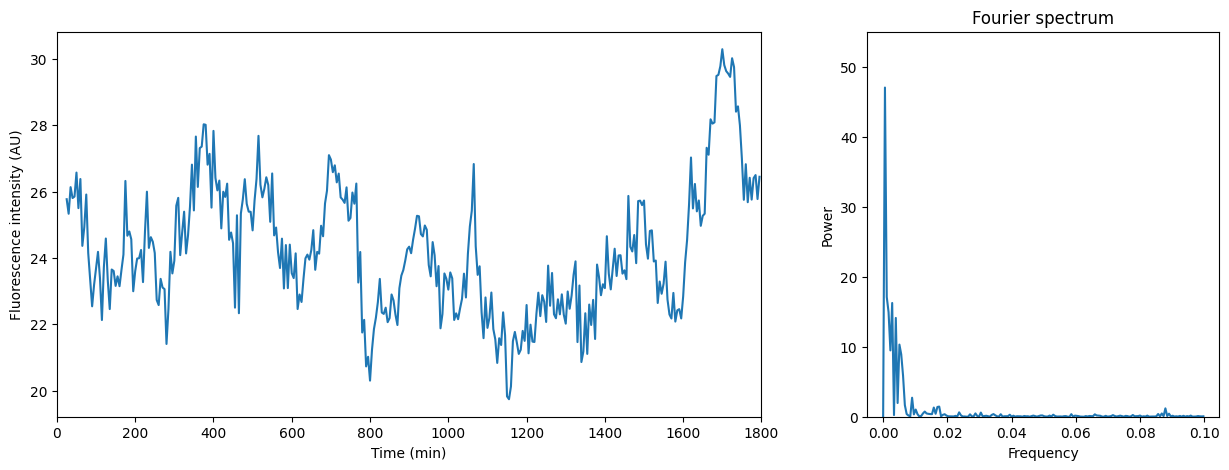
\includegraphics[width=\textwidth]{fft_raw}
   \caption{
   }
   \label{fig:analysis-filter-raw}
  \end{subfigure}

  \begin{subfigure}[htpb]{0.8\textwidth}
   \centering
   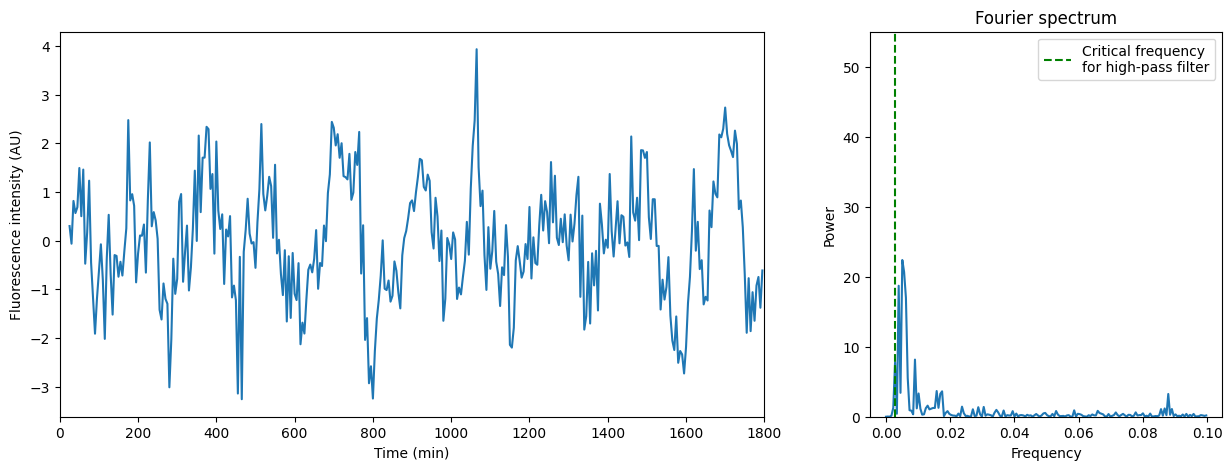
\includegraphics[width=\textwidth]{fft_butterworth}
   \caption{
   }
   \label{fig:analysis-filter-butterworth}
  \end{subfigure}

  \begin{subfigure}[htpb]{0.8\textwidth}
   \centering
   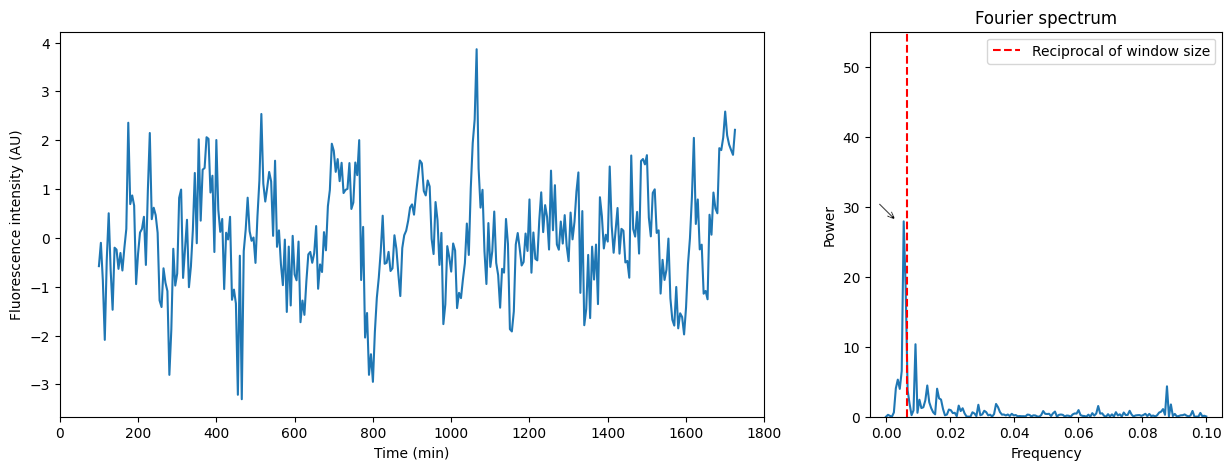
\includegraphics[width=\textwidth]{fft_slidingwindow_edit}
   \caption{
   }
   \label{fig:analysis-filter-movavg}
  \end{subfigure}

  \caption[
    Time series and Fourier spectra corresponding to
    a sample raw time series of flavin autofluorescence,
    the time series processed by a high-pass Butterworth filter, and
    the time series detrended using a moving average.
  ]{
    (Left panels) Time series and (right panels) Fourier spectra corresponding to
    \textbf{(\ref{fig:analysis-filter-raw})}
    a sample raw time series of flavin autofluorescence,
    \textbf{(\ref{fig:analysis-filter-butterworth})}
    the time series processed by a high-pass Butterworth filter with a critical frequency \SI{2.86d-3}{\minute^{-1}}, and
    \textbf{(\ref{fig:analysis-filter-movavg})}
    the time series detrended using a moving average (window size 30 time points).
    Arrow ($\searrow$) indicates artefact.
  }
  \label{fig:analysis-filter}
\end{figure}

To demonstrate the use of a method that modifies the frequency profile of time series to remove trends, Figs.\ \ref{fig:analysis-filter-raw}--\ref{fig:analysis-filter-butterworth} show how a time series and its Fourier spectrum changes after the application of a high-pass Butterworth filter with a critical frequency of \SI{2.86d-3}{\minute^{-1}}, corresponding to a period of \SI{350}{\minute}.
Defining a signal filter offers direct control over frequencies.
The critical frequency was chosen as a reasonable upper limit of periods of the yeast metabolic cycle, based on my observations in single-cell microfluidics experiments.
Defining the critical frequency in this way excludes the possibility of metabolic cycles that have very long periods in favour of emphasising metabolic oscillations of an expected frequency.

To show how sliding-window methods may adversely affect the frequency profile of time series when used for detrending, I computed the Fourier spectrum of time series detrended using the moving average method.
Sliding-window methods are common in detrending biological time series.
For example, \textcite{cunyHighresolutionMassMeasurements2022} used a moving average: a constant, defined sliding window to smooth time series of yeast cell mass during growth.
%\textcite{papagiannakisAutonomousMetabolicOscillations2017} fitted a smoothing spline to their single-cell fluorescence data of the yeast metabolic cycle, then divided the data points by the smoothing spline to detrend their data; the specific mathematical method used to define the smoothing spline was unclear in their study.
%
Fig.\ \ref{fig:analysis-filter-movavg} shows that the moving average method introduced an artefact in the frequency spectrum near the reciprocal of the window size and decreases the number of time points.


\section{Visualising groups in the dataset}
\label{sec:analysis-clustering}

To identify structures in datasets of time series, I implemented UMAP, a dimension reduction method, and modularity clustering, a graph-based clustering method.
Such data visualisation methods are important because the structures they show may identify differences between groups that are biologically relevant --- for example, subpopulations of oscillations with similar properties.
Previous efforts in using computational methods to identify groups in a set of biological time series include using $k$-means clustering to identify clusters of transcript cycling patterns that correspond to phases of the YMC \parencite{tuLogicYeastMetabolic2005}, development of a method to cluster featurised multivariate time series based of videos of human motion \parencite{wangStructureBasedStatisticalFeatures2007}, and using signal entropy to featurise fMRI signals followed by modularity clustering to partition the signals into brain regions.

To demonstrate the data visualisation methods, I used time series of flavin autofluorescence oscillations from one experiment with both the wild-type BY4741 strain ($n=206$) and the mutant \textit{zwf1$\Delta$} strain ($n=425$).
These time series had time points sampled every \SI{5}{\minute} in the experiment, for a total of 163 time points.
I manually labelled the time series to indicate whether they were oscillatory or not, with 142 of the 206 BY4741 time series classed as oscillatory and 224 of the 425 \textit{zwf1$\Delta$} classed as oscillatory.


\subsection{UMAP}
\label{subsec:analysis-clustering-umap}

UMAP \parencite{mcinnesUMAPUniformManifold2020} is an unsupervised dimension reduction method that can be used to visualise structure in a dataset.
Specifically, UMAP aims to find a manifold structure of the input observations and compute a low-dimensional embedding that preserves the topological structure of the manifold.
This embedding thus serves as coordinates to plot the data onto a low-dimensional space.

\begin{figure}
  \centering
  \begin{subfigure}[t]{0.5\textwidth}
  \centering
    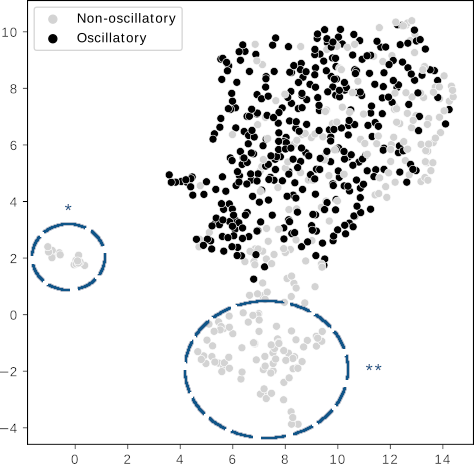
\includegraphics[width=\linewidth]{umap_single_is20016_2_edit2.png}
    \caption{
    }
    \label{fig:umap-osc}
  \end{subfigure}%
  \begin{subfigure}[t]{0.5\textwidth}
  \centering
    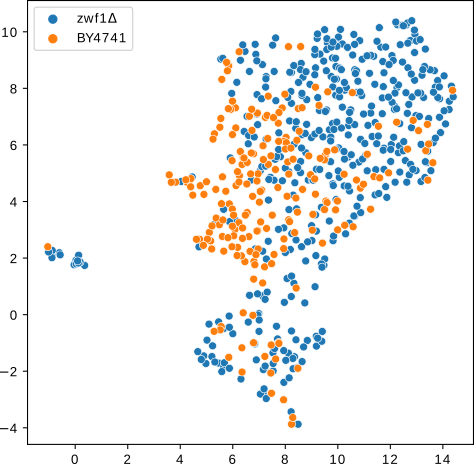
\includegraphics[width=\linewidth]{umap_single_is20016_1_edit.png}
    \caption{
    }
    \label{fig:umap-strain}
  \end{subfigure}

  \caption[
      UMAP embedding of a dataset of time series featurised using \textit{catch22}.
    ]{
      UMAP embedding ($n=5$, $\mathrm{min\_dist} = 0.5$, $d=2$, Euclidean distance as the metric) of a dataset of time series featurised using \textit{catch22}.
      Each node represents a time series, coloured either by
      \textbf{(\ref{fig:umap-osc})}
      whether each is oscillatory or not, human-labelled ($\ast$ and $\ast \ast$ indicating two groups of non-oscillatory nodes of interest), or by
      \textbf{(\ref{fig:umap-strain})}
      strain (`BY4741' or `\textit{zwf1$\Delta$}').
    }
  \label{fig:umap}
\end{figure}

To evaluate whether UMAP was able to discover a structure within the BY4741 \& \textit{zwf1$\Delta$} dataset that corresponded to meaningful divisions, I featurised the time series with \textit{catch22}, then used UMAP to compute two-dimensional embeddings.
Fig.\ \ref{fig:umap-osc} demonstrates that UMAP suggested a small group of non-oscillatory time series that differed markedly from the rest ($\ast$ in figure), and a larger group that was more similar to oscillatory time series ($\ast \ast$ in figure).
In addition, Fig.\ \ref{fig:umap-strain} demonstrates that UMAP suggested that the BY4741 time series were more similar to each other.
In contrast, \textit{zwf1$\Delta$} occupied larger regions of the embedding space.
These embeddings agreed with my observation that time series from the \textit{zwf1$\Delta$} strain had a larger variety of shapes and oscillation quality than the BY4741 strain.
Thus, UMAP may have potential to separate oscillatory and non-oscillatory time series, or time series of different shapes.


\begin{figure}
  \centering
    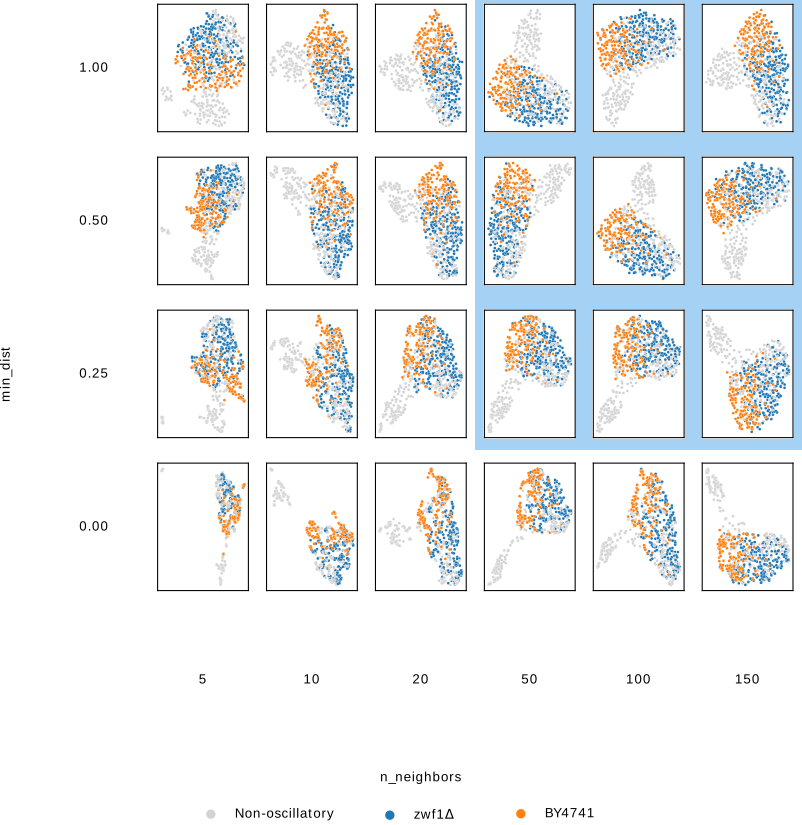
\includegraphics[width=0.9\linewidth]{umap_grid_is20016_edit3.png}
    \caption[
      Grid search of UMAP hyperparameters.
    ]{
      Grid search of UMAP hyperparameters: number of neighbours along the horizontal axis and minimum distance along the vertical axis.
      Data points are coloured according to category: grey indicates non-oscillatory time series, blue indicates oscillatory time series from \textit{zwf1$\Delta$} cells, and orange indicates oscillatory time series from BY4741 cells.
    }
  \label{fig:umap-gridsearch}
\end{figure}

To improve the visualisation, I performed a grid search of the $n$ and $\mathrm{min\_dist}$ UMAP hyperparameters (Appendix~\ref{append:analysis-umap}) to find the best combination.
Fig.\ \ref{fig:umap-gridsearch} suggests that $50 \leq n \leq 150$ and $0.25 \leq \mathrm{min\_dist} \leq 1$ resulted in a good separation between the BY4741 and \textit{zwf1$\Delta$} nodes.
In addition, non-oscillatory time series were consistently displayed into groups separate from the rest as the hyperparameters were varied.


\subsection{Graph-based clustering}
\label{subsec:analysis-clustering-graphclustering}

Modularity clustering is a mathematical method that partitions a graph into groups to optimise a `modularity' value, defined so that the method finds a trade-off between maximising the connections within a cluster and minimising the connections between clusters \parencite{newmanModularityCommunityStructure2006}.
This optimisation problem is computationally difficult, so approximations such as the Louvain algorithm are needed for large networks \parencite{blondelFastUnfoldingCommunities2008}, with the Leiden algorithm \parencite{traagLouvainLeidenGuaranteeing2019} subsequently developed to ensure that communities are well-connected and to provide an optimum number of communities.
Furthermore, the intrinsic scale of modularity scales with the square root of the number of connections in the network; therefore, if the network is large, there is a large resolution limit, preventing a modularity clustering algorithm from detecting small-scale structures \parencite{fortunatoResolutionLimitCommunity2007,traagNarrowScopeResolutionlimitfree2011}.
To remedy this, algorithms that implement a resolution parameter ($\gamma$), were devised; the value of this parameter thus controls the scale at which communities are detected \parencite{reichardtDetectingFuzzyCommunity2004,kumpulaLimitedResolutionComplex2007}.

\begin{figure}
  \centering
  \begin{subfigure}[t]{0.5\textwidth}
  \centering
    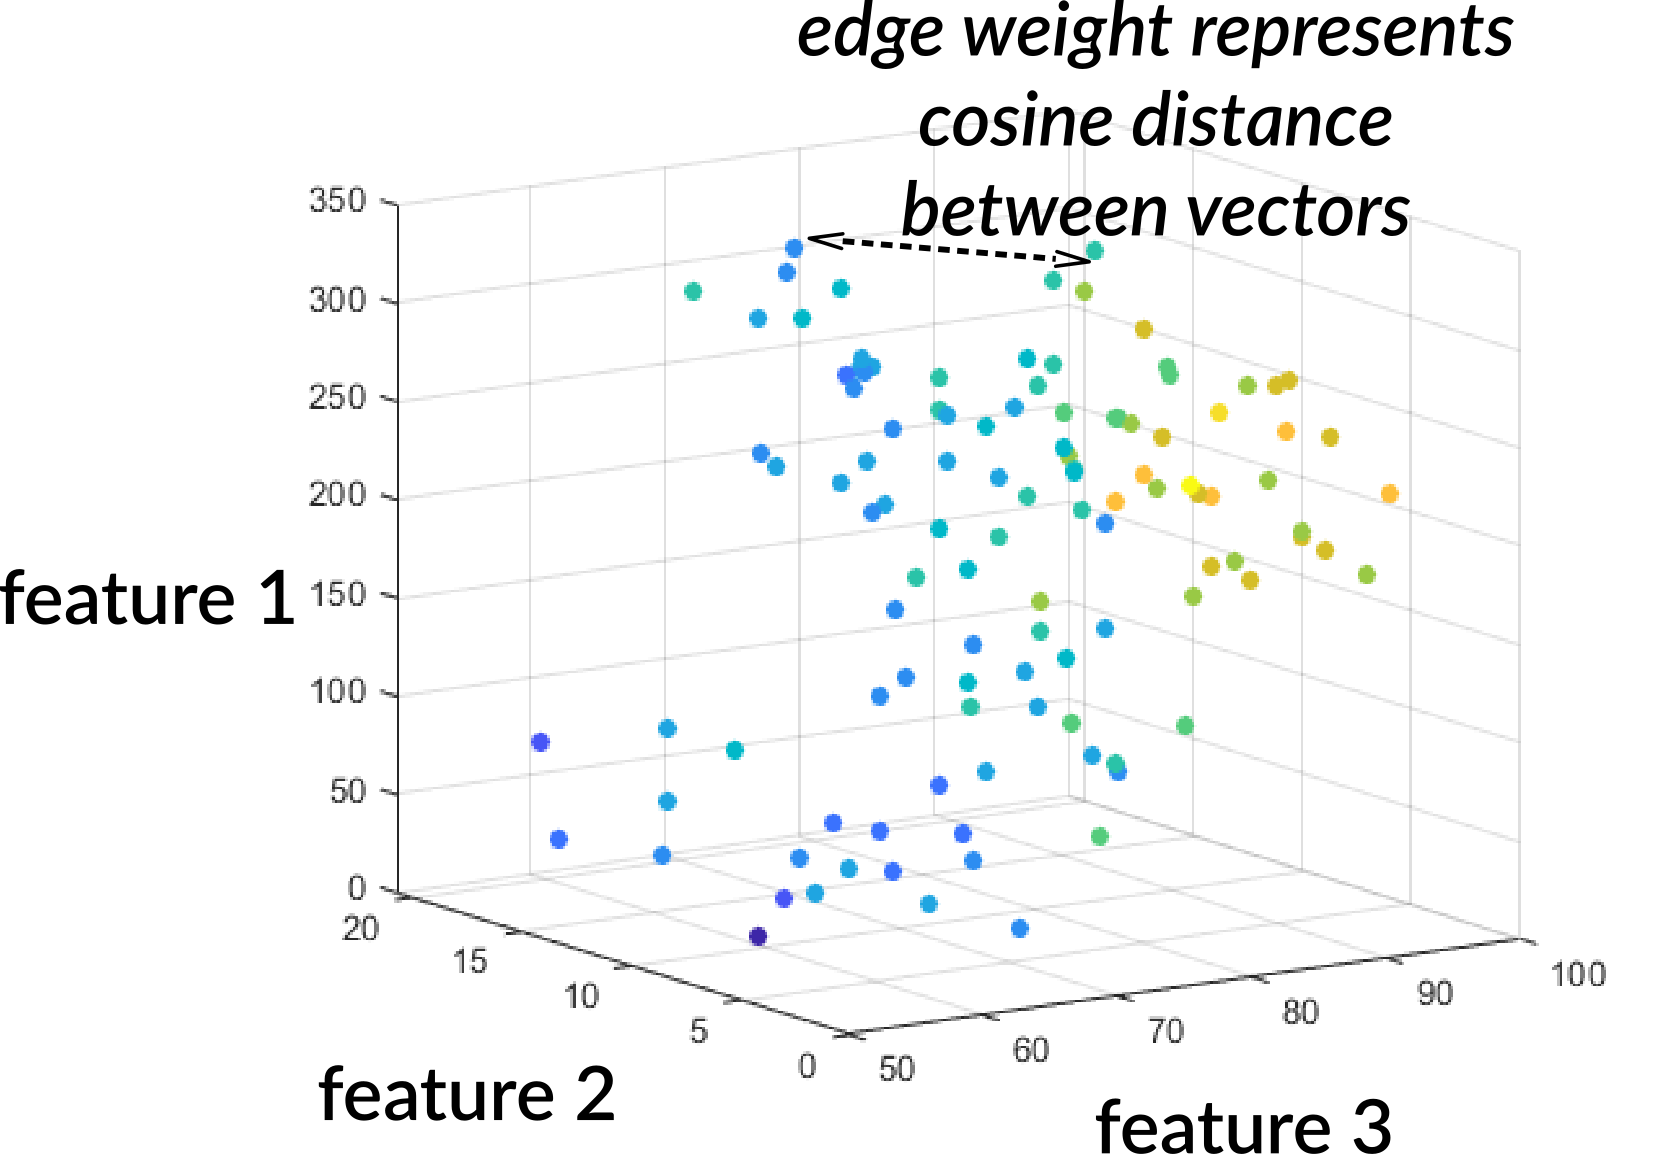
\includegraphics[width=\linewidth]{graph_representation}
    \caption{
    }
    \label{fig:analysis-clustering-modclust-graph}
  \end{subfigure}

  \begin{subfigure}[t]{0.45\textwidth}
  \centering
    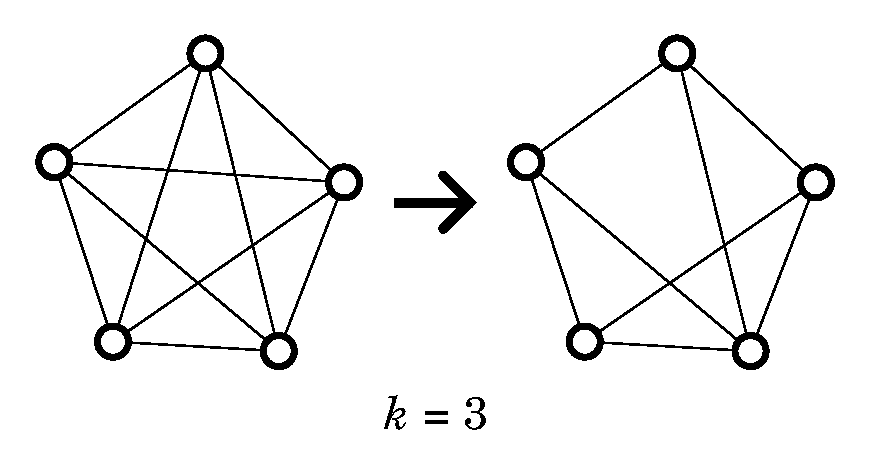
\includegraphics[width=\linewidth]{pruning}
    \caption{
    }
    \label{fig:analysis-clustering-modclust-prune}
  \end{subfigure}%
  \begin{subfigure}[t]{0.45\textwidth}
  \centering
    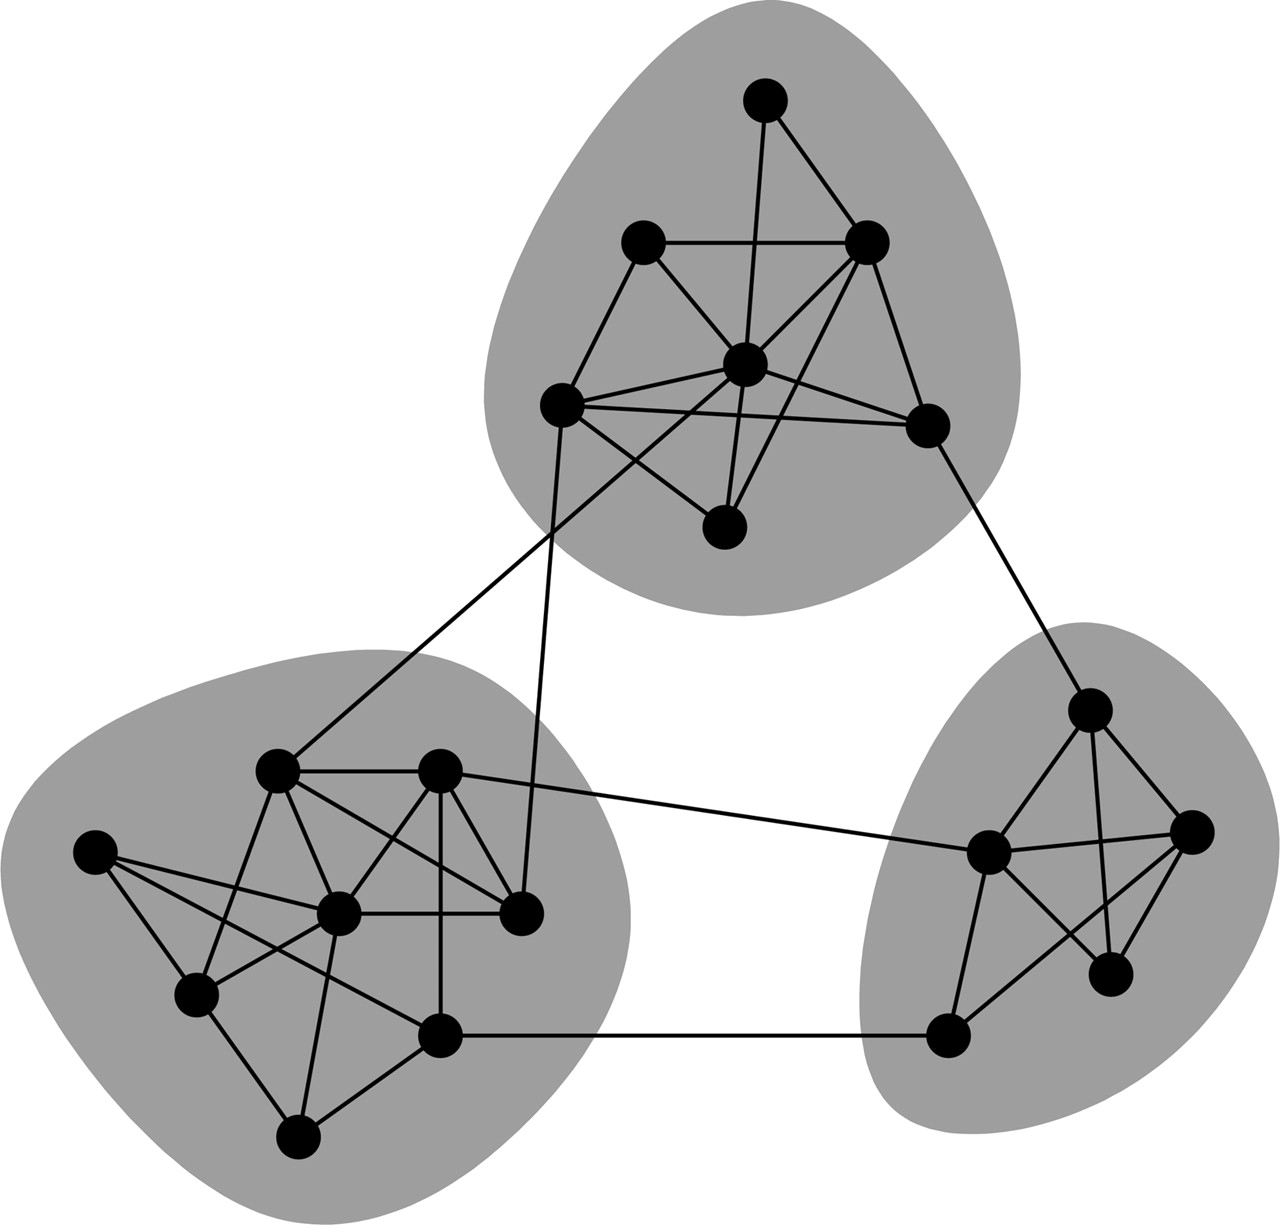
\includegraphics[width=\linewidth]{newmanModularityCommunityStructure2006_1}
    \caption{
    }
    \label{fig:analysis-clustering-modclust-modclust}
  \end{subfigure}

  \caption[
    Process of preparing a dataset of time series for modularity clustering.
  ]{
    Process of preparing a dataset of time series for modularity clustering.
    \textbf{(\ref{fig:analysis-clustering-modclust-graph})}
    Constructing a graph representation: each time series was featurised and the cosine distances in feature space became edge weights.
    \textbf{(\ref{fig:analysis-clustering-modclust-prune})}
    Pruning the complete graph so that each node had at least the $k$ nearest neighbours.
    \textbf{(\ref{fig:analysis-clustering-modclust-modclust})}
    Modularity clustering, using the Leiden algorithm \parencite{traagLouvainLeidenGuaranteeing2019}, to identify communities.
    \ref{fig:analysis-clustering-modclust-modclust} adapted from \textcite{newmanModularityCommunityStructure2006}.
    In all subfigures, data are synthetic and only serve to illustrate the process.
  }
  \label{fig:analysis-clustering-modclust}
\end{figure}

To assess the performance of a graph-based clustering method in identify clusters in time series data, I represented a dataset of time series as a graph before using modularity clustering to identify clusters.
Fig.\ \ref{fig:analysis-clustering-modclust} illustrates this process, specifically:
\begin{enumerate}
  \item \emph{Constructing a graph representation:}
        Each time series was represented as a vector of features in $n$-dimensional space, where $n$ is the length of the vector.
        Here, I represented each time series with a vector of 22 features using \textit{catch22}.
        The cosine distances between each pair of vector was computed, and became the edge weights of a complete graph with each time series as a node.
  \item \emph{Pruning:}
        The complete graph was pruned by deleting edges, so that each node was connected to at least the $k$ nearest neighbours.
        I used $k=10$.
  \item \emph{Modularity clustering:}
        Modularity clustering was performed on the graph to partition the pruned graph into communities.
        In this step, I used the Leiden algorithm \parencite{traagLouvainLeidenGuaranteeing2019}.
\end{enumerate}


\begin{figure}[htbp]
  \centering
  \begin{subfigure}[t]{0.5\textwidth}
  \centering
    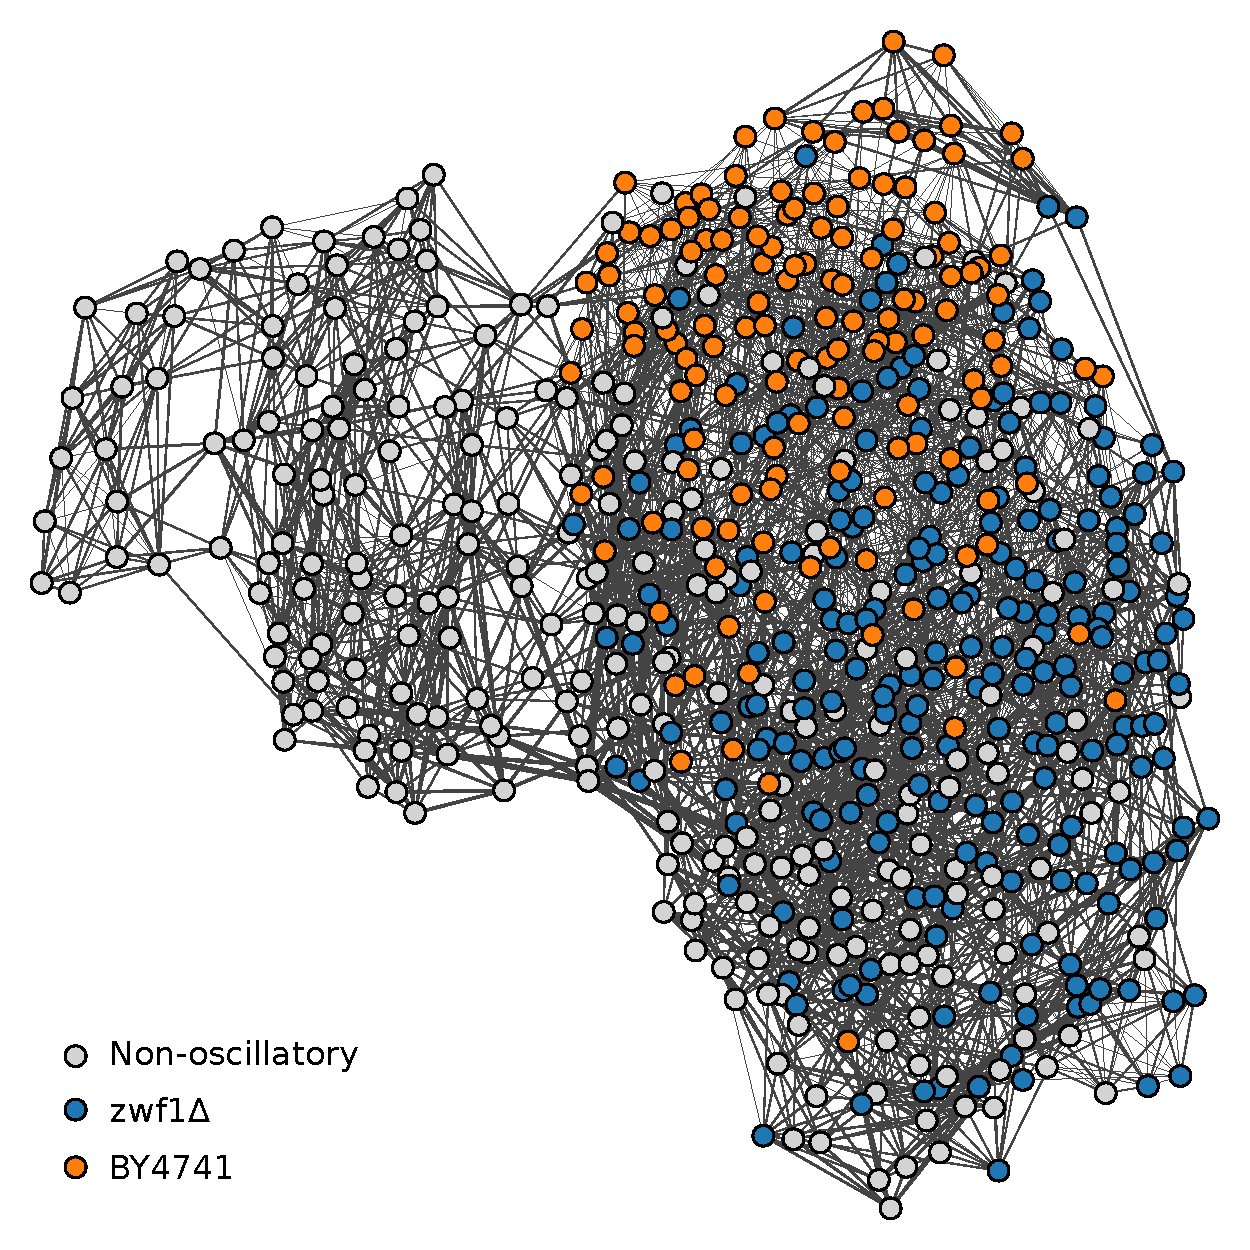
\includegraphics[width=\linewidth]{graphclust_combined_is20016_edit1.pdf}
    \caption{
    }
    \label{fig:graphclustering-combined}
  \end{subfigure}

  % \begin{subfigure}[t]{0.5\textwidth}
  % \centering
  %   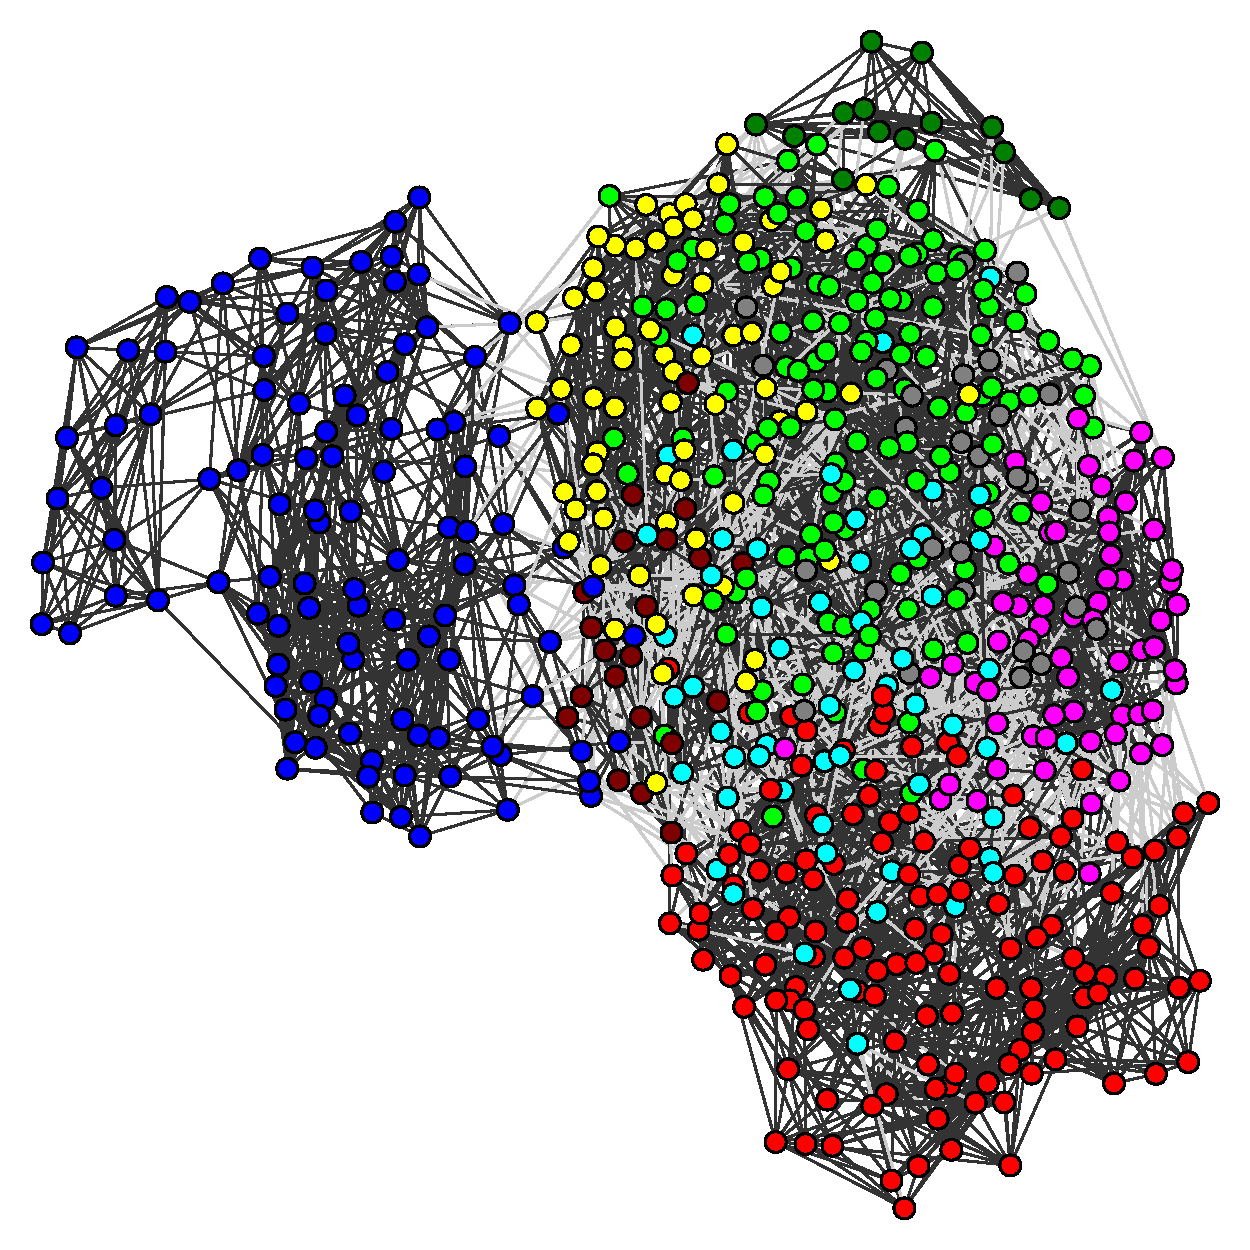
\includegraphics[width=\linewidth]{graphclust_leiden_is20016.pdf}
  %   \caption{
  %   }
  %   \label{fig:graphclustering-leiden}
  % \end{subfigure}

  \begin{subfigure}[t]{0.33\textwidth}
  \centering
    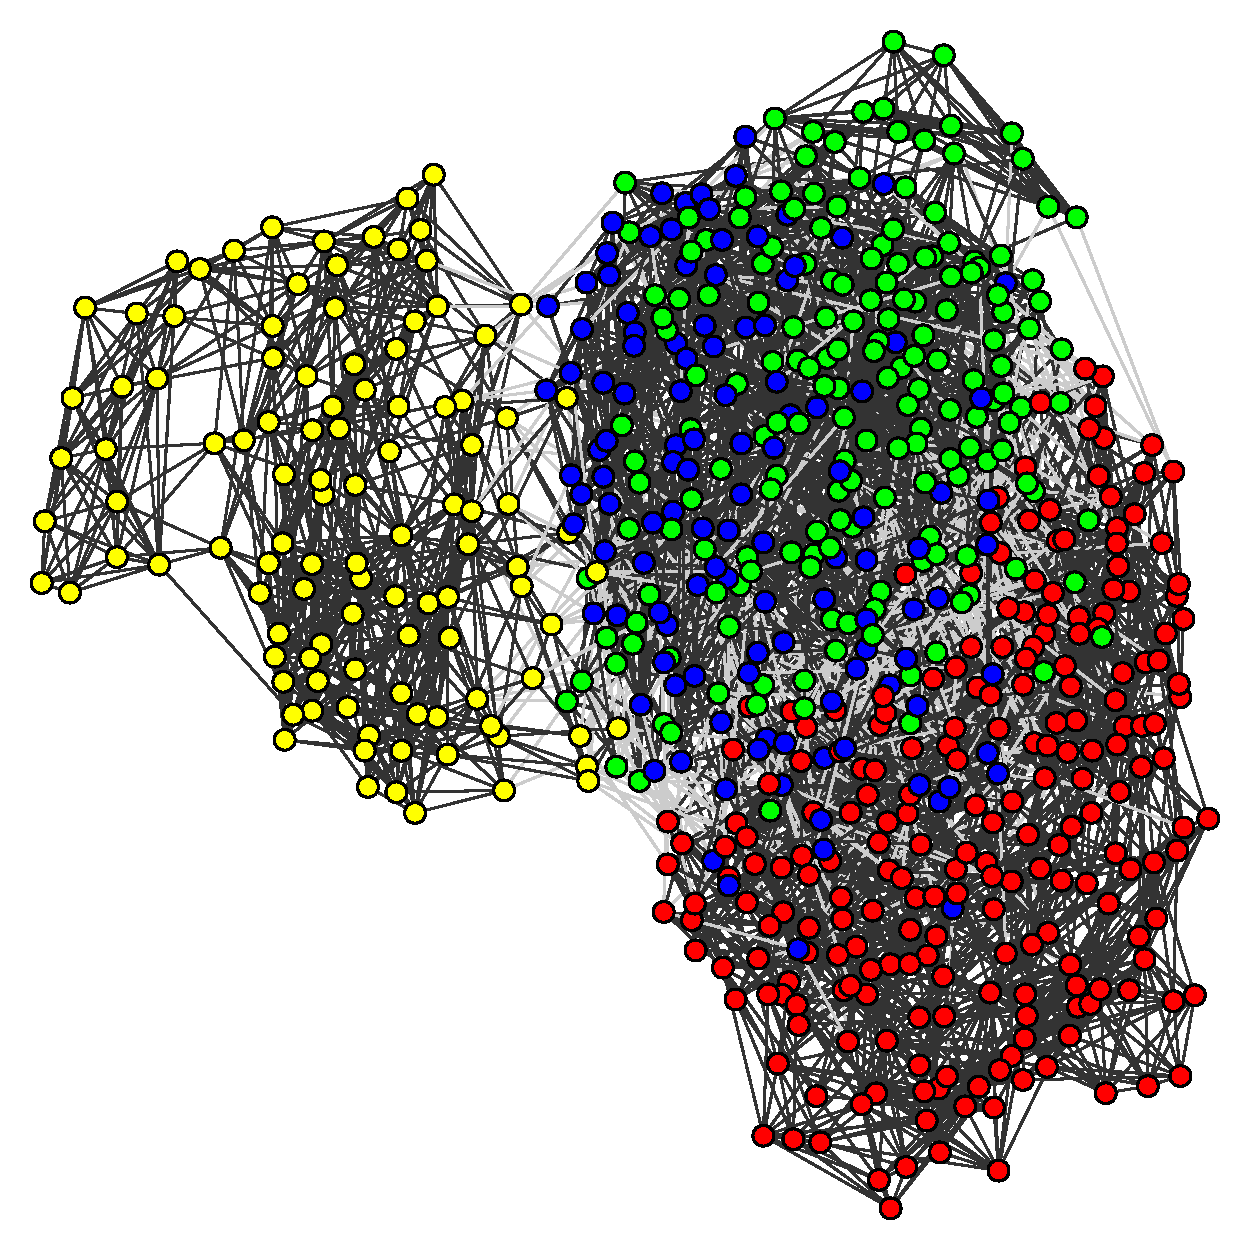
\includegraphics[width=\linewidth]{graphclust_cpm_00p010_is20016.pdf}
    \caption{
    }
    \label{fig:graphclustering-cpm_00p010}
  \end{subfigure}%
  \begin{subfigure}[t]{0.33\textwidth}
  \centering
    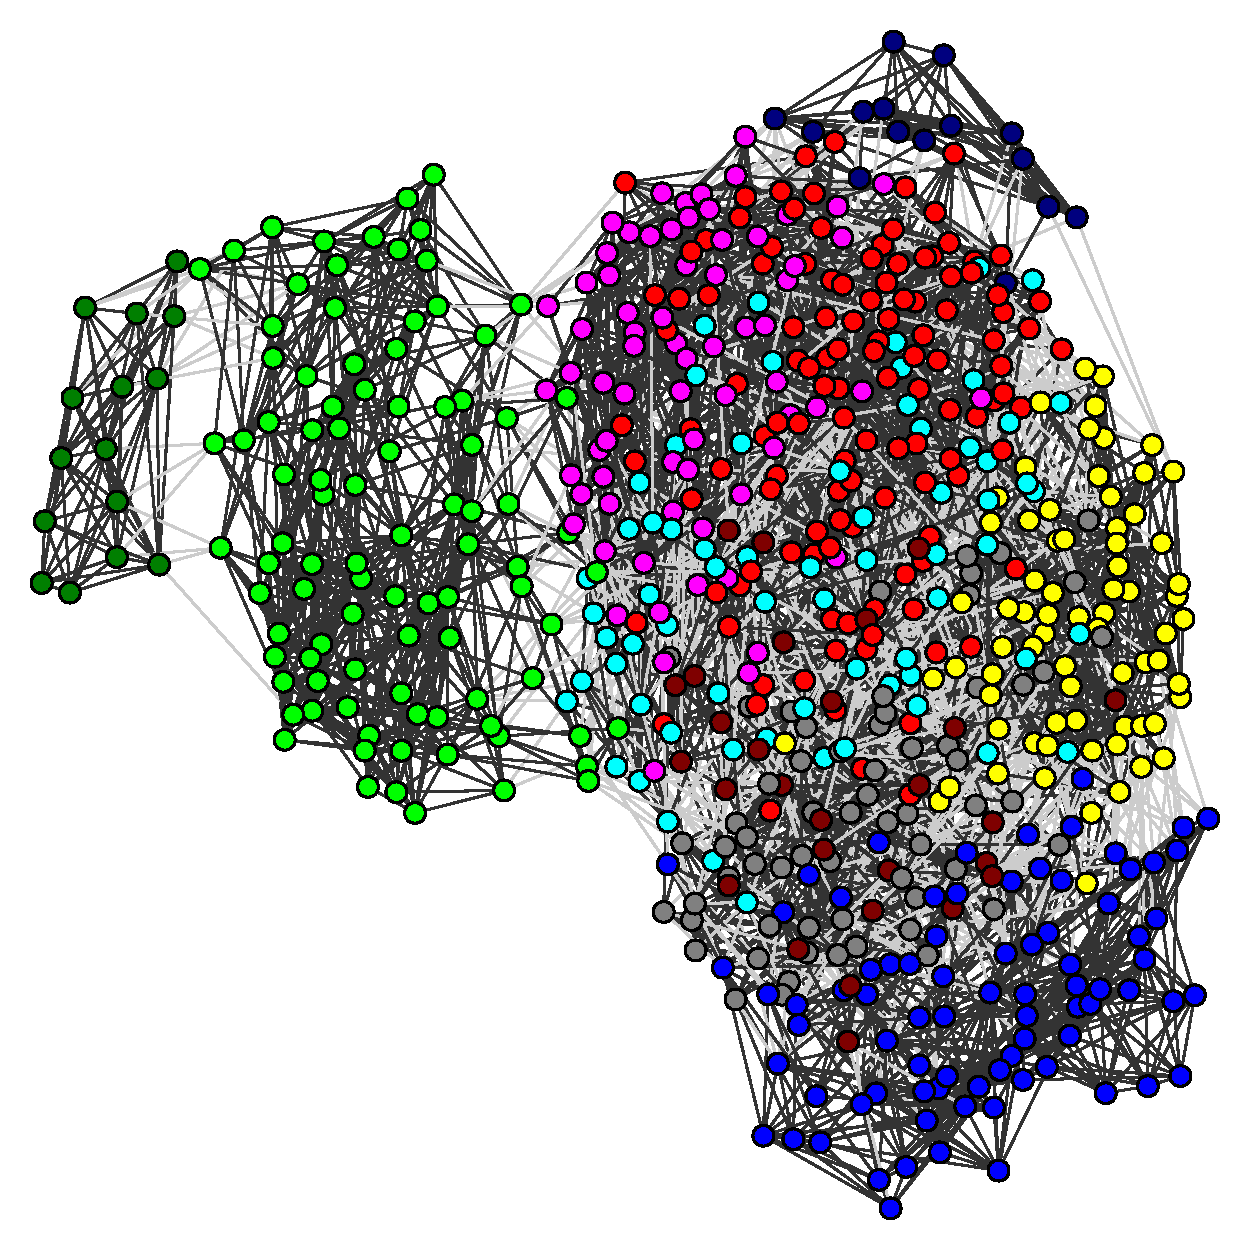
\includegraphics[width=\linewidth]{graphclust_cpm_00p020_is20016.pdf}
    \caption{
    }
    \label{fig:graphclustering-cpm_00p020}
  \end{subfigure}%
  \begin{subfigure}[t]{0.33\textwidth}
  \centering
    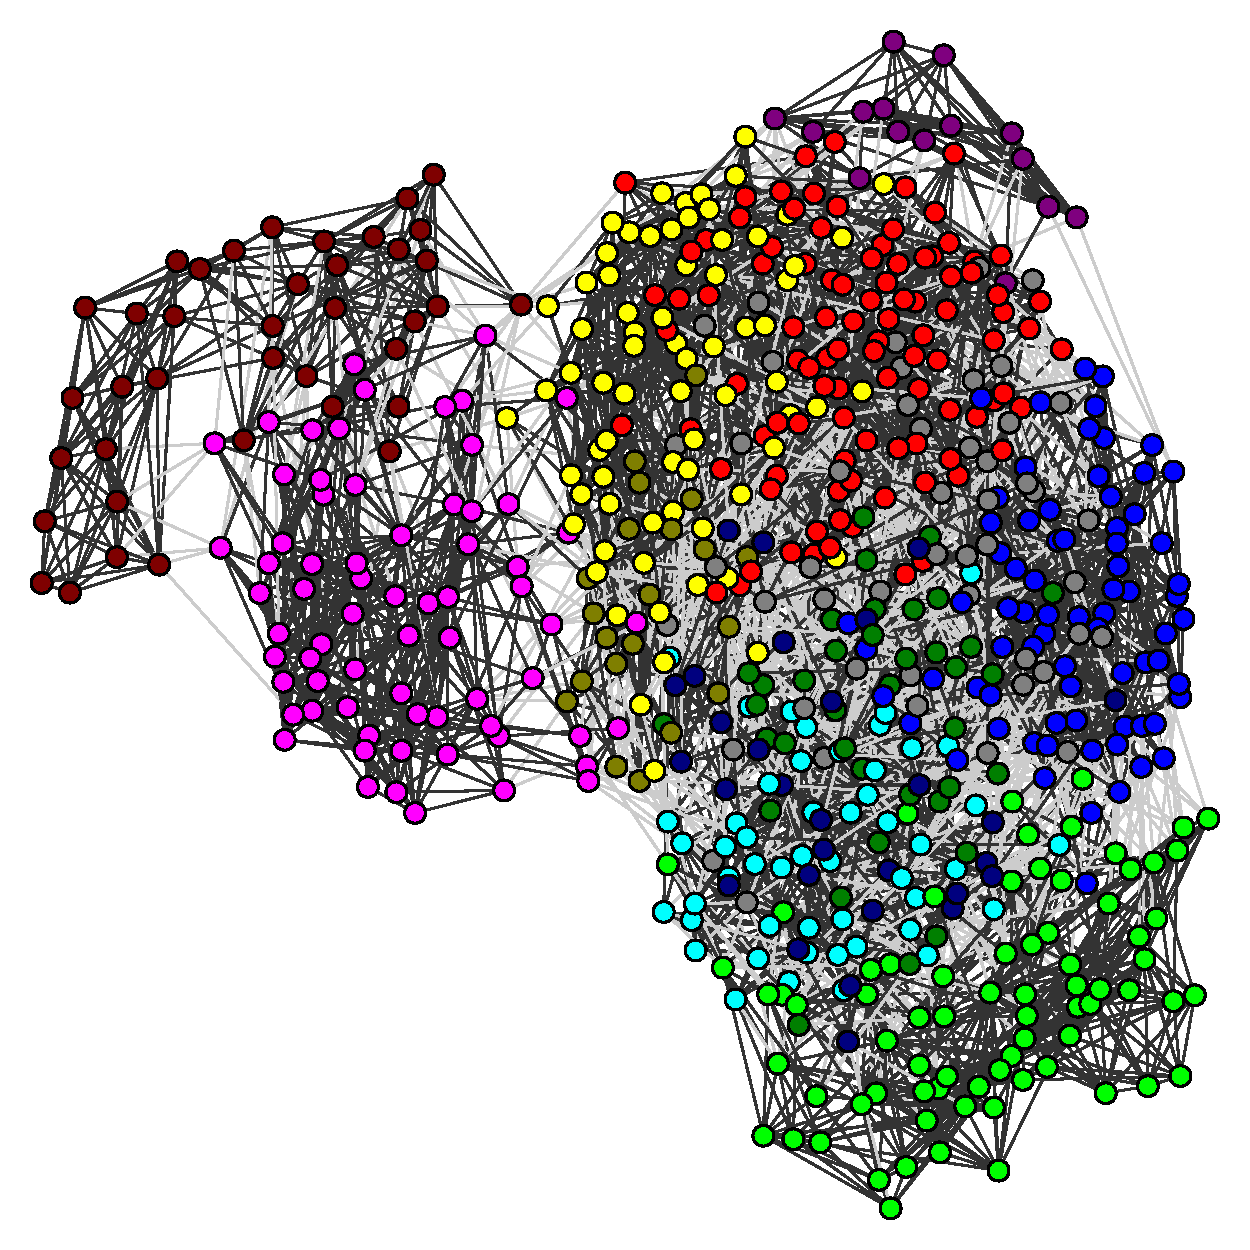
\includegraphics[width=\linewidth]{graphclust_cpm_00p030_is20016.pdf}
    \caption{
    }
    \label{fig:graphclustering-cpm_00p030}
  \end{subfigure}

  \caption[
    Pruned graph of BY4741 and \textit{zwf1$\Delta$} time series from the same experiment.
  ]{
    Pruned graph of BY4741 and \textit{zwf1$\Delta$} time series from the same experiment.
    \textbf{(\ref{fig:graphclustering-combined})}
    Nodes coloured by group: grey, non-oscillatory; blue, oscillatory \textit{zwf1$\Delta$}; orange, oscillatory BY4741.
    Thickness of edges represent edge weights, scaled by similarity found by cosine distances.
    % \textbf{(\ref{fig:graphclustering-leiden})}
    % Nodes coloured by community (out of 10) as optimised by the Leiden algorithm.
    % Edges within a community are in black, while edges between communities are in light grey.
    Additionally, nodes coloured by community as found by the constant Potts model \parencite{traagNarrowScopeResolutionlimitfree2011} as the resolution parameter ($\gamma$) was varied:
    \textbf{(\ref{fig:graphclustering-cpm_00p010})} $\gamma = 0.01$ (4 communities),
    \textbf{(\ref{fig:graphclustering-cpm_00p020})} $\gamma = 0.02$ (10 communities), and
    \textbf{(\ref{fig:graphclustering-cpm_00p030})} $\gamma = 0.03$ (12 communities).
  }
  \label{fig:graphclustering}
\end{figure}

Fig.\ \ref{fig:graphclustering-combined} shows that construction of a pruned graph based on similarities between time series highlights two groups of non-oscillatory time series.
Subsequently, Figs.\ \ref{fig:graphclustering-cpm_00p010}--\ref{fig:graphclustering-cpm_00p030} show the resolution parameter ($\gamma$) controls the number of communities detected.
Non-oscillatory time series were assigned to a separate group when $\gamma = 0.01$, and the two sub-groups of non-oscillatory time series were separated when $\gamma = 0.02$; however, $\gamma = 0.03$, the divisions changed.
The Leiden algorithm \parencite{traagLouvainLeidenGuaranteeing2019} suggested 10 as the optimal number of communities, which was realised by $\gamma = 0.02$.
For all $\gamma$ values, modularity clustering was able to further show communities among the oscillatory time series.
However, such communities did not divide cleanly along the division between BY4741 and \textit{zwf1$\Delta$} cells, suggesting that time series features alone were not able to divide these two strains.
This agreed with my observation that some oscillatory \textit{zwf1$\Delta$} time series resembled BY4741 time series (Fig.\ \ref{fig:analysis-sample-zwf1}).

\begin{figure}
  \centering
  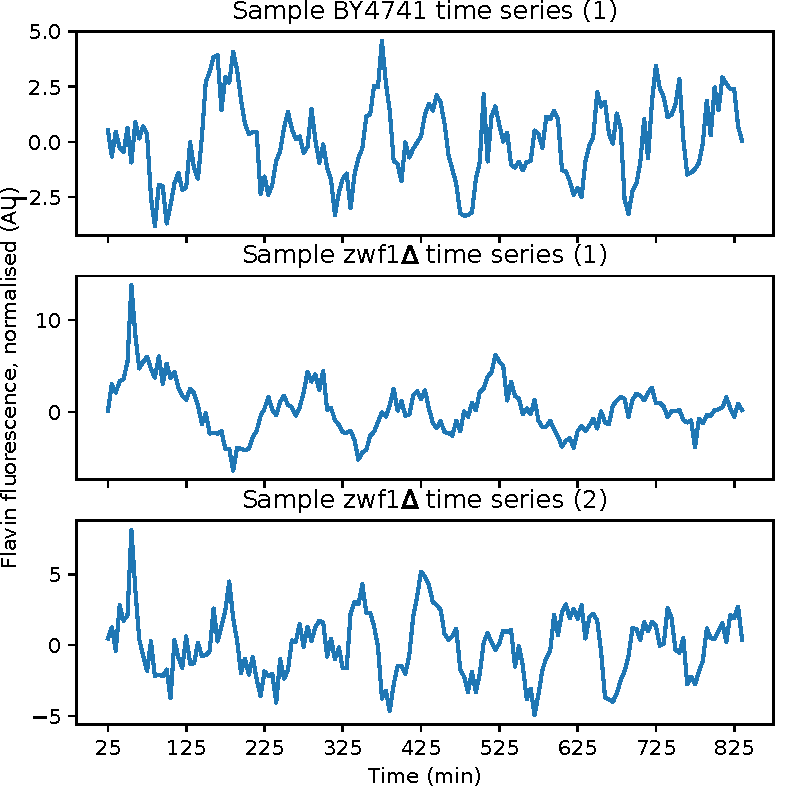
\includegraphics[width=0.6\linewidth]{sample_ts_zwf1.pdf}

  \caption[
    Sample time series from BY4741 and \textit{zwf1$\Delta$} cells.
  ]{
    Sample time series from BY4741 and \textit{zwf1$\Delta$} cells.
    \textit{zwf1$\Delta$} sample 1 does not resemble the BY4741 sample, while \textit{zwf1$\Delta$} sample 2 does.
  }
  \label{fig:analysis-sample-zwf1}
\end{figure}

% PLOT AVERAGE TIME SERIES FROM EACH COMMUNITY?

In sum, the general agreement between UMAP and modularity clustering shows that the BY4741 \& \textit{zwf1$\Delta$} dataset had internal structure defined by rhythmicity of time series.
However, it was not clear from the UMAP whether there are sub-populations among the BY4741 and \textit{zwf1$\Delta$} time series whose members exhibit similar types of oscillations.
In contrast, while modularity clustering suggests that such sub-populations can be found based on connectivity between nodes, the number of sub-populations depends on the value of a resolution parameter.


\section{Detection of rhythmicity}
\label{sec:analysis-classification}

To identify metabolic cycles from flavin autofluorescence signals, it is important to have a systematic method to determine whether a time series is oscillatory.
To determine the time series classification method that is most appropriate for my data, I compared a spectral method, a model-fitting method, and a machine learning method.


\subsection{Rhythmicity detection using spectral methods}
\label{subsec:analysis-classification-spectral}

In order to classify oscillatory and non-oscillatory time series, I modified a classifier based on a spectral method that included a statistical test (Methods Section~\ref{subsec:methods-computational-periodogram}).
This classifier was based on \textcite{glynnDetectingPeriodicPatterns2006a}, which described a method that employed the peak power from the Lomb-Scargle periodogram \parencite{lombLeastsquaresFrequencyAnalysis1976} to rank time series by the quality of oscillation and to perform a statistical test to determine whether a time series is oscillatory or non-oscillatory \parencite{scargleStudiesAstronomicalTime1982}, as shown by Eqs.\ \ref{eq:lsp-pval}--\ref{eq:lsp-khat}.

\begin{figure}[htbp]
  \centering
  \begin{subfigure}[t]{0.65\textwidth}
  \centering
    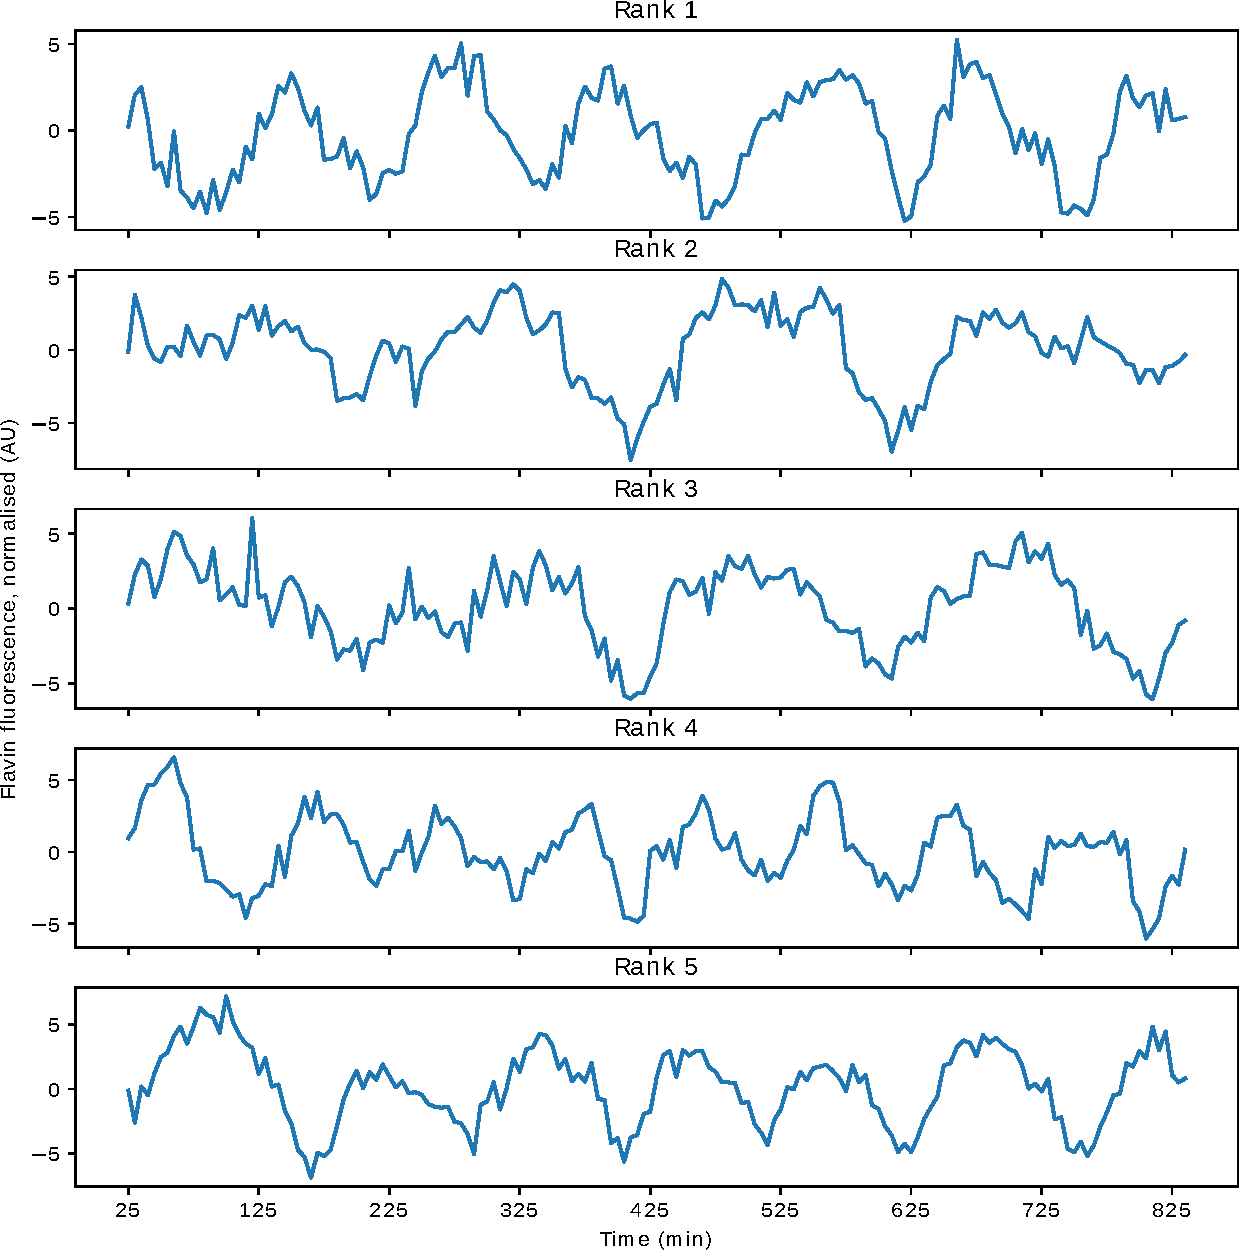
\includegraphics[width=\linewidth]{glynn_is20016_1_edit.pdf}
    \caption{
    }
    \label{fig:glynn-best-ts}
  \end{subfigure}%
  \begin{subfigure}[t]{0.35\textwidth}
  \centering
    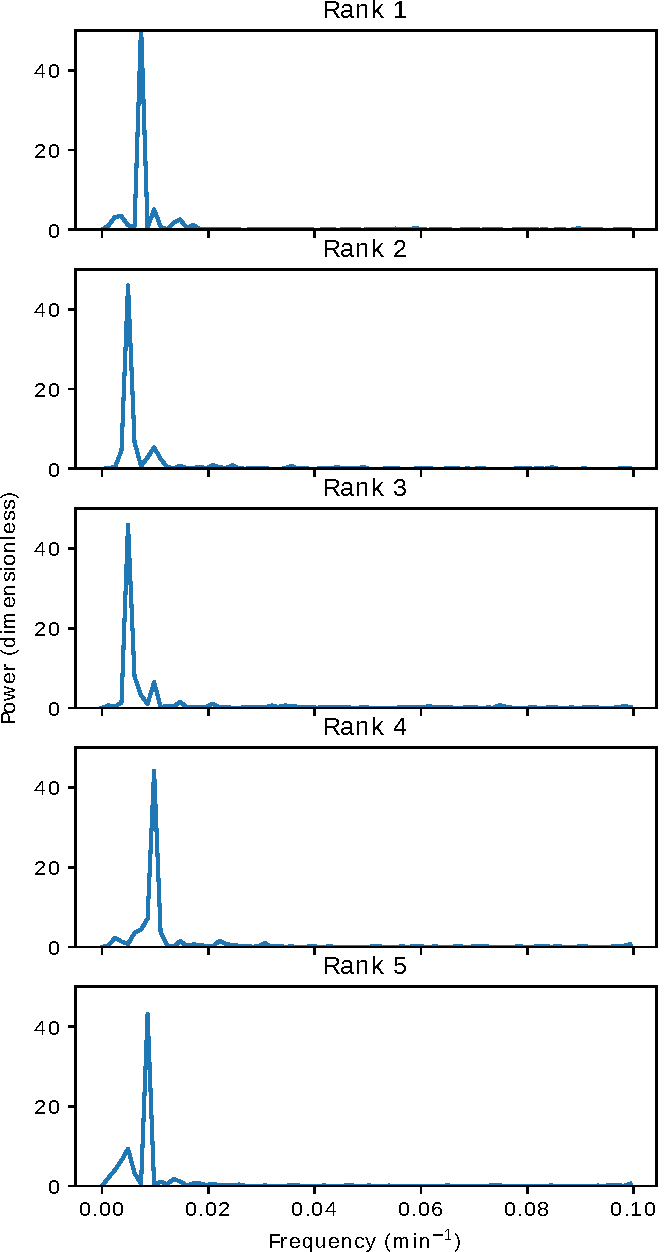
\includegraphics[width=\linewidth]{glynn_is20016_2_edit.pdf}
    \caption{
    }
    \label{fig:glynn-best-ps}
  \end{subfigure}

  \caption[
    Best five time series in the \textit{zwf1$\Delta$} dataset and
    their periodograms,
    ranked by the quality of oscillation based on the maximum power in the periodogram \parencite{glynnDetectingPeriodicPatterns2006a}
  ]{
    \textbf{(\ref{fig:glynn-best-ts})}
    Best five time series in the \textit{zwf1$\Delta$} dataset and
    \textbf{(\ref{fig:glynn-best-ps})}
    their periodograms,
    ranked by the quality of oscillation based on the maximum power in the periodogram \parencite{glynnDetectingPeriodicPatterns2006a}.
  }
  \label{fig:glynn-best}
\end{figure}

\begin{figure}[htbp]
  \centering
  \begin{subfigure}[t]{0.65\textwidth}
  \centering
    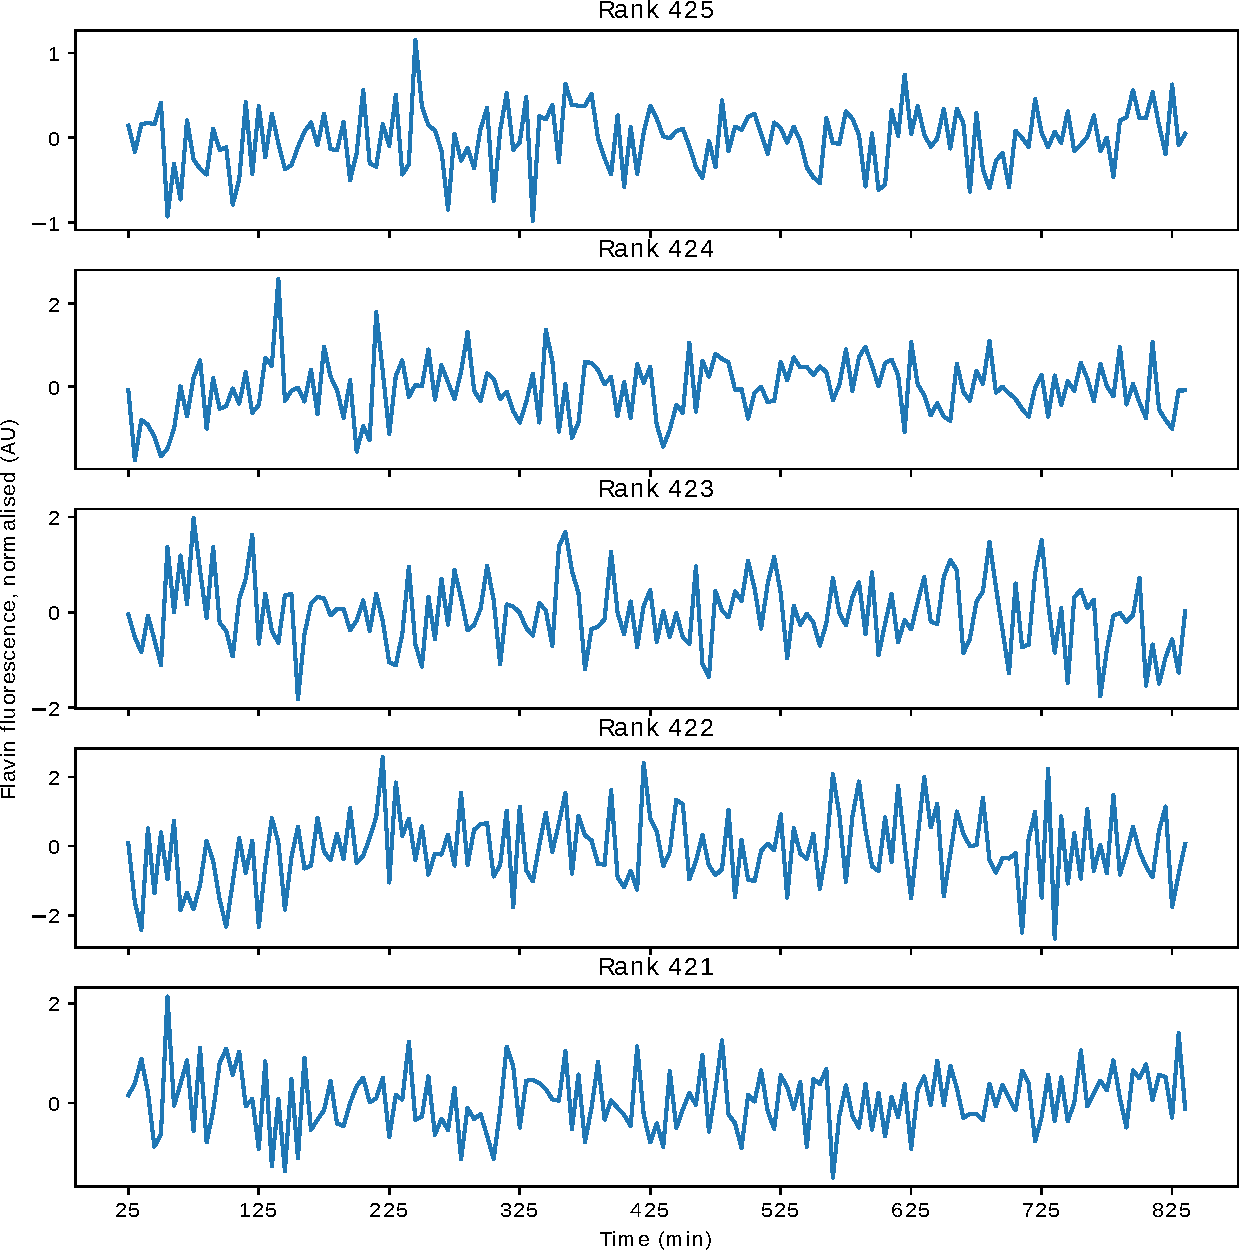
\includegraphics[width=\linewidth]{glynn_is20016_3_edit.pdf}
    \caption{
    }
    \label{fig:glynn-worst-ts}
  \end{subfigure}%
  \begin{subfigure}[t]{0.35\textwidth}
  \centering
    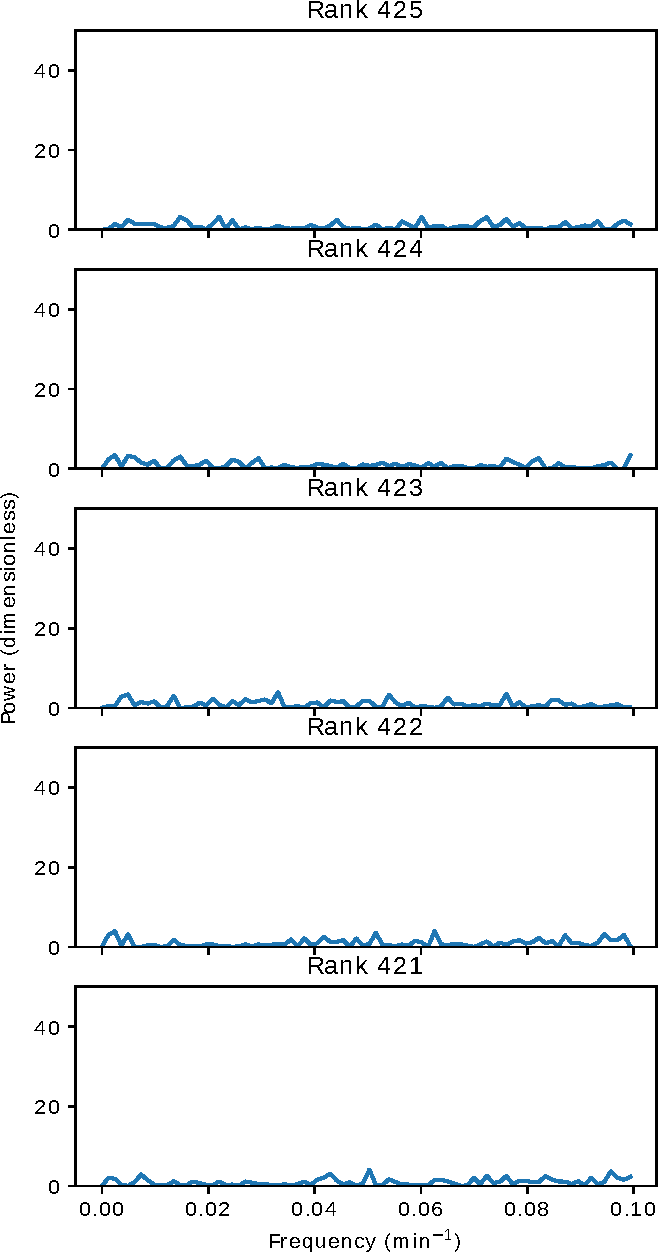
\includegraphics[width=\linewidth]{glynn_is20016_4_edit.pdf}
    \caption{
    }
    \label{fig:glynn-worst-ps}
  \end{subfigure}

  \caption[
    Worst five time series in the \textit{zwf1$\Delta$} dataset and
    their periodograms,
    ranked by the quality of oscillation based on the maximum power in the periodogram \parencite{glynnDetectingPeriodicPatterns2006a}
  ]{
    \textbf{(\ref{fig:glynn-worst-ts})}
    Worst five time series in the \textit{zwf1$\Delta$} dataset and
    \textbf{(\ref{fig:glynn-worst-ps})}
    their periodograms,
    ranked by the quality of oscillation based on the maximum power in the periodogram \parencite{glynnDetectingPeriodicPatterns2006a}.
  }
  \label{fig:glynn-worst}
\end{figure}

Figs.\ \ref{fig:glynn-best}--\ref{fig:glynn-worst} suggest that the best- and worst-ranked time series by the quality of their oscillatory signals conformed to subjective judgements of quality.
Highest-ranked time series resembled sinusoids and therefore led to periodograms with a strong power corresponding to the frequency of the sinusoid that would model the time series.
Conversely, lowest-ranked time series resembled white noise and led to periodograms with power equally spread across all frequencies, thus bringing down the height of the highest peak.
However, some time series with irregular oscillations based on visual inspection (Fig.\ \ref{fig:glynn-best}; ranks 2, 3) were given higher ranks than those with more regular oscillations based on visual inspection, thus calling into question the reliability of the ranking method.

\begin{figure}
  \centering
  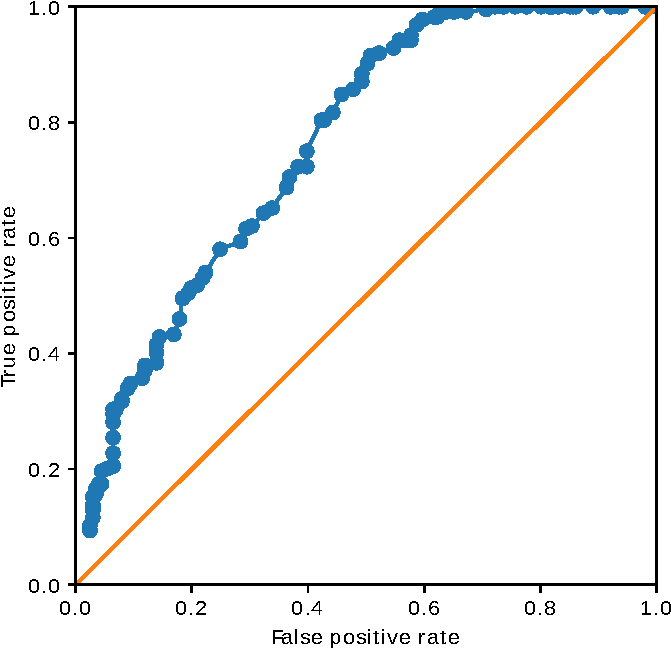
\includegraphics[width=0.5\textwidth]{glynn_is20016_5_edit.pdf}
  \caption[
    ROC curve of classifier based on \textcite{glynnDetectingPeriodicPatterns2006a}.
  ]{
    ROC curve of classifier based on \textcite{glynnDetectingPeriodicPatterns2006a} as the false discovery rate was varied.
    The true positive rate and false positive rates were evaluated based on manual scoring of the \textit{zwf1$\Delta$} dataset.
  }
  \label{fig:glynn-roc}
\end{figure}

To detect rhythmicity in one time series, \textcite{glynnDetectingPeriodicPatterns2006a} calculates the probability of the null hypothesis that a peak in the periodogram occurs due to chance.
When extended across a population of time series, rhythmicity detection by this method thus becomes a task of testing multiple hypotheses.
\textcite{glynnDetectingPeriodicPatterns2006a} thus proposed controlling the false discovery rate, defined as the proportion of cases in which the null hypothesis is true among all hypotheses in which the test is declared significant (see Methods, Section~\ref{subsec:methods-computational-periodogram}, specifically Eq.\ \ref{eq:lsp-khat}).
Controlling the false discovery rate thus controls the expected proportion of oscillations that are classified as oscillatory.

To assess the performance of this method as a classifier for rhythmicity detection, Fig.\ \ref{fig:glynn-roc} shows the receiver operating characteristic (ROC) curve, created as the false discovery rate was varied.
The area under the ROC curve ($A = 0.762$) suggests that the classifier performed modestly well, especially for a large ($n=425$) dataset of time series with a large variety of quality of oscillations.


\subsection{Rhythmicity detection using model fitting}
\label{subsec:analysis-classification-ar}

To assess the performance of a time series classification method based on the autoregressive model, I implemented the method described by \textcite{jiaFrequencyDomainAnalysis2020}, used to characterise synthetic time series of stochastic, oscillatory gene expression in a dividing cell.
In the implementation of the autoregressive model used by \textcite{jiaFrequencyDomainAnalysis2020}, each data point was expressed as a linear combination of a number of data points that precede it, and model parameters led to an analytical solution for the periodogram, thus giving an advantage over the low-resolution Fourier spectrum (Methods Section~\ref{subsec:methods-computational-ar}).
The resulting power spectra fell into four categories, one of which corresponded to a lack of oscillations, characterised by an absence of a local maximum in the power spectrum (Fig.\ \ref{fig:analysis-ar-classification}).
This method thus allows computing the frequency of the oscillation from the location of the peak in the periodogram and quality of the oscillation from the height of the peak.

\begin{figure}
  \centering
  \begin{subfigure}[htpb]{0.6\textwidth}
   \centering
   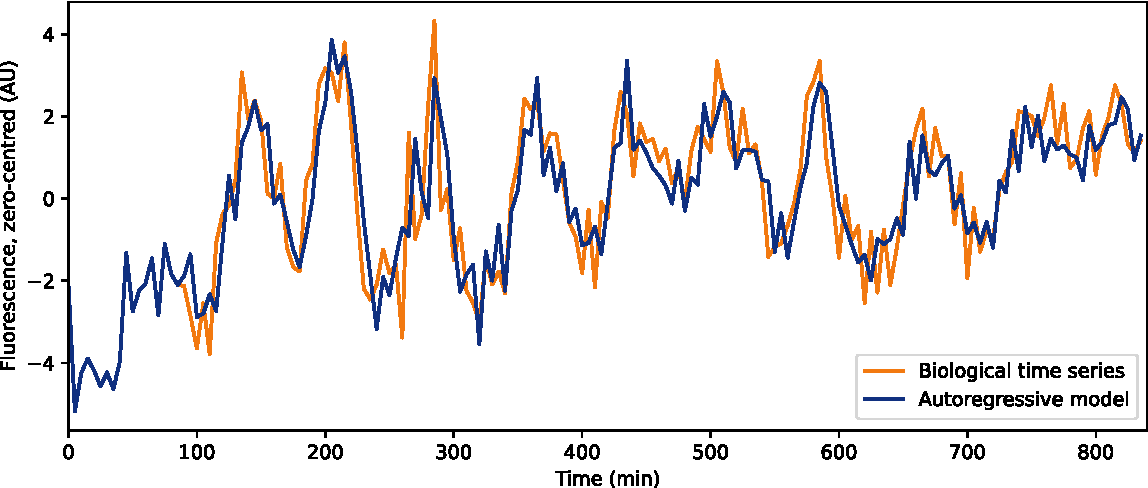
\includegraphics[width=\textwidth]{timeseries_example_for_ar_edit}
   \caption{
   }
   \label{fig:analysis-ar-timeseries}
  \end{subfigure}%
  \begin{subfigure}[htpb]{0.4\textwidth}
   \centering
   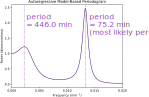
\includegraphics[width=\textwidth]{ar}
   \caption{
   }
   \label{fig:analysis-ar-periodogram}
  \end{subfigure}

  \caption[
    Sample time series, with a fitted autoregressive model computed according to \textcite{jiaFrequencyDomainAnalysis2020}.
  ]{
    \textbf{(\ref{fig:analysis-ar-timeseries})}
    Sample time series (orange), with a fitted autoregressive model (blue) of order 18 computed according to \textcite{jiaFrequencyDomainAnalysis2020}.
    \textbf{(\ref{fig:analysis-ar-periodogram})}
    Periodogram defined based on parameters of the autoregressive model.
    % The presence of a peak of height greater than 1 indicates that the time series is oscillatory.
    % Furthermore, the locations of peaks estimate the period of oscillation in the original time series.
  }
  \label{fig:analysis-ar}
\end{figure}


\begin{figure}
  \centering
  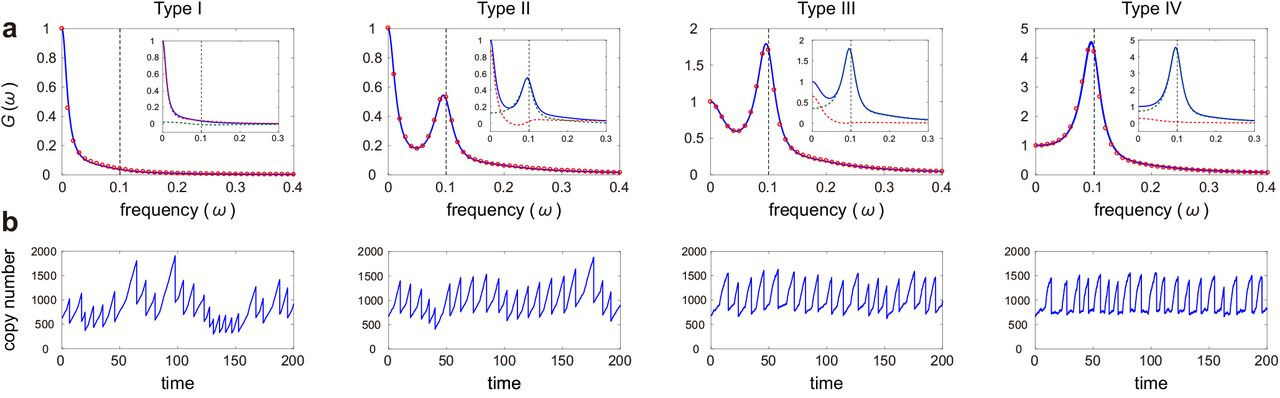
\includegraphics[width=1.0\textwidth]{jiaFrequencyDomainAnalysis2020_2ab_adapted}
  \caption[
    Power spectra analytically derived from fitting an autoregressive model to time series can be divided into four types.
  ]{
    Power spectra (a) analytically derived from fitting an autoregressive model to time series (b) can be divided into four types.
    Type I lacks a local maximum and is denoted as lacking oscillations.
    Figure adapted from \textcite{jiaFrequencyDomainAnalysis2020}.
  }
  \label{fig:analysis-ar-classification}
\end{figure}

Fig.\ \ref{fig:analysis-ar} shows that the autoregressive model was able to correctly identify a time series as oscillatory at a period of \SI{75.2}{\minute}, as evidenced by the location of a peak in the periodogram that the model predicted.


\begin{table}
  \centering
  % https://tex.stackexchange.com/a/20295
  \begin{tabular}{l|l|c|c|c}
    \multicolumn{2}{c}{}&\multicolumn{2}{c}{Predicted by AR model}&\\
    \cline{3-4}
    \multicolumn{2}{c|}{}&Positive&Negative&\multicolumn{1}{c}{Total}\\
    \cline{2-4}
    \multirow{2}{*}{Human-defined labels}& Positive & 141 & 83 & 224\\
    \cline{2-4}
    & Negative & 124 & 77 & 201\\
    \cline{2-4}
    \multicolumn{1}{c}{} & \multicolumn{1}{c}{Total} & \multicolumn{1}{c}{265} & \multicolumn{1}{c}{160} & \multicolumn{1}{c}{425}\\
  \end{tabular}
  \caption[
    Confusion matrix to evaluate the performance of using the autoregressive model \parencite{jiaFrequencyDomainAnalysis2020} to detect rhythmicity.
  ]{
    Confusion matrix to evaluate the performance of using the autoregressive model \parencite{jiaFrequencyDomainAnalysis2020} to detect rhythmicity in the \textit{zwf1$\Delta$} dataset.
  }
  \label{tab:analysis-ar-confusion-matrix}
\end{table}

To assess the performance of the use of the autoregressive model for rhythmicity detection across a dataset, I extended this method across the \textit{zwf1$\Delta$} dataset, treating Type I power spectra (Fig.\ \ref{fig:analysis-ar-classification}) as non-oscillatory.
The confusion matrix (table~\ref{tab:analysis-ar-confusion-matrix}) suggests that the method leads to poor performance (precision = 0.532, recall = 0.629, no-skill classifier: precision = recall = 0.527, see Methods Section~\ref{subsec:methods-computational-precision-recall} for definitions), as it classed a large proportion of time series as non-oscillatory.


\subsection{Rhythmicity detection using machine learning}
\label{subsec:analysis-classification-ml}

As an alternative to the mathematical methods previously discussed, I trained a support vector classifier to classify oscillatory and non-oscillatory time series from the \textit{zwf1$\Delta$} cells (appendix \ref{append:analysis-ml}).

To ensure that the dynamic ranges of the fluorescence signals do not affect rhythmicity detection, I normalised each time series $x_{i}(t_{1}), \ldots , x_{i}(t_{j}), \ldots , x_{i}(t_{N})$ to produce a processed time series $z_{i}(t_{1}), \ldots , z_{i}(t_{j}), \ldots , z_{i}(t_{N})$ as follows:

\begin{equation}
  z_{i}(t_{j}) = \frac{x_{i}(t_{j}) - \mu_{i}}{\sigma_{i}}
  \label{eq:analysis-stdscore}
\end{equation}

where $\mu_{i}$ is the mean value of $x_{i}$ computed across all time points, and $\sigma_{i}$ is the standard deviation of $x_{i}$ computed across all time points.
As a result, each normalised time series $z_{i}$ has a mean of 0 and a standard deviation of 1.
From this input data, 75\% of the time series formed the training set.

\begin{figure}
  \centering
  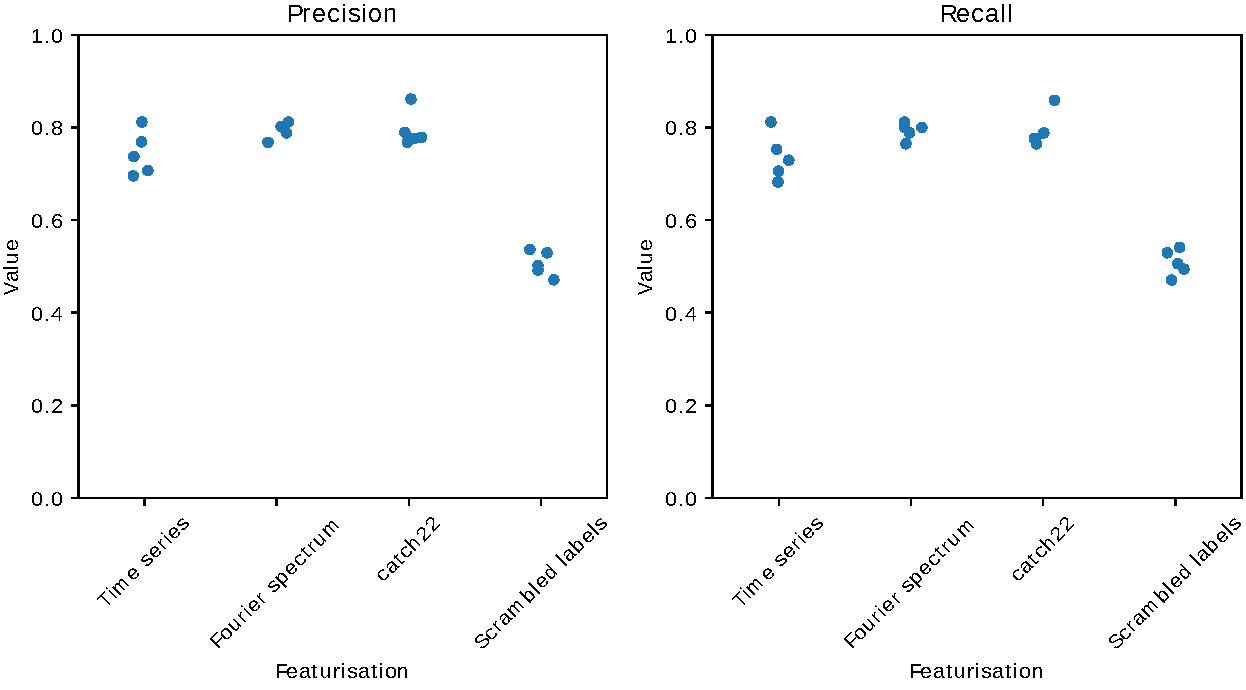
\includegraphics[width=0.9\textwidth]{svm_feat_compare_edit.pdf}
  \caption[
    Precision and recall from five-fold cross-validation of support vector classifiers trained using different featurisation methods.
  ]{
    (Left) Precision and (right) recall from five-fold cross-validation of support vector classifiers trained using different featurisation methods:
    using the time points as features,
    using the power values in the Fourier spectrum as features,
    and using \emph{catch22} features.
    As a control, the oscillatory and non-oscillatory labels were randomly assigned to the time series and the time points were used as features.
  }
  \label{fig:analysis-precision-recall}
\end{figure}

% \begin{figure}
%   \centering
%   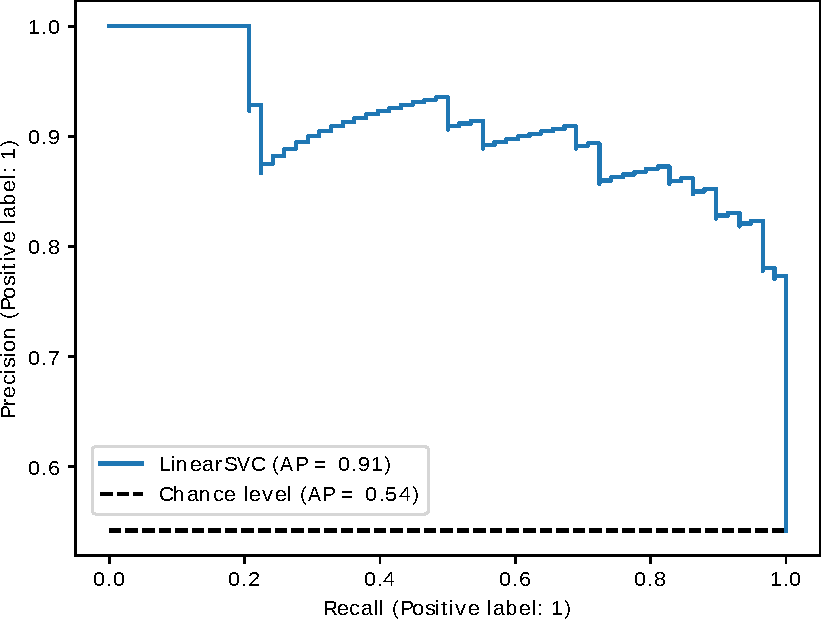
\includegraphics[width=0.7\textwidth]{svm_1_edit.pdf}
%   \caption[
%     Precision-recall curve of binary classifier
%   ]{
%     Precision-recall curve of binary classifier, using \textit{catch22} for featurisation and with a support vector classifier architecture (radial bias kernel, $\gamma = 1/22$, $C = 1$).
%   }
%   \label{fig:analysis-svc-pr}
% \end{figure}

To determine the most effective way to featurise the data, I computed the precision and recall (defined in Methods Section~\ref{subsec:methods-computational-precision-recall}) of support vector classifiers trained on data featurised using different methods.
All support vector classifiers were trained using a radial bias kernel, a kernel coefficient $\gamma = 1/N$, where $N$ is the number of features, and a regularisation parameter $C = 10$.
Fig.\ \ref{fig:analysis-precision-recall} suggests that featurisation using \textit{catch22} and the Fourier spectrum gave comparably high performances, as evidenced by high precision and recall, and with a low degree of overfitting, as evidenced by a small variation of both metrics across the rounds of cross-validation.
%To evaluate the performance of the \textit{catch22}-based classifier, Fig. \ref{fig:analysis-svc-pr} shows the precision-recall curve of the classifier, which suggests a good performance.


\begin{figure}
  \centering
  \begin{subfigure}[htpb]{0.5\textwidth}
   \centering
   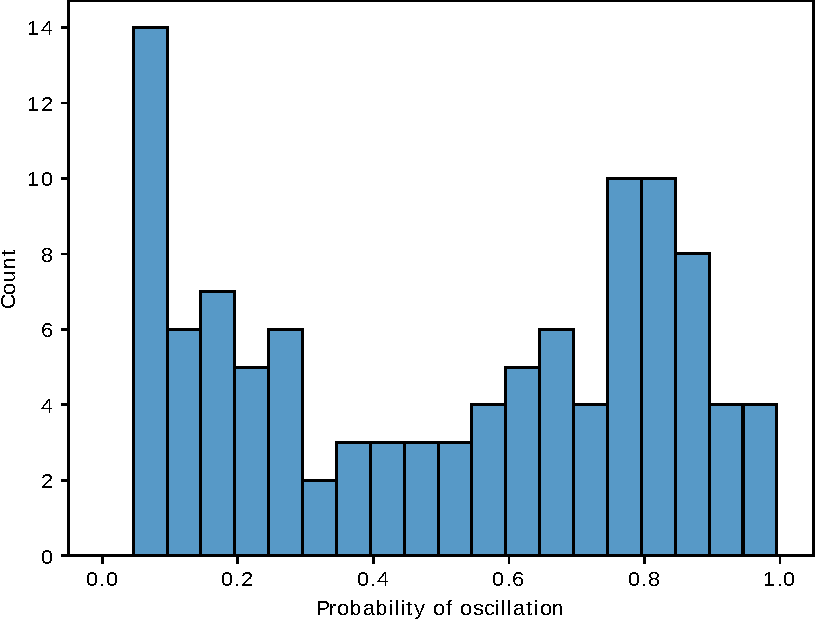
\includegraphics[width=\textwidth]{svm_2_edit.pdf}
   \caption{
   }
   \label{fig:analysis-svc-proba-histogram-model}
  \end{subfigure}%
  \begin{subfigure}[htpb]{0.5\textwidth}
   \centering
   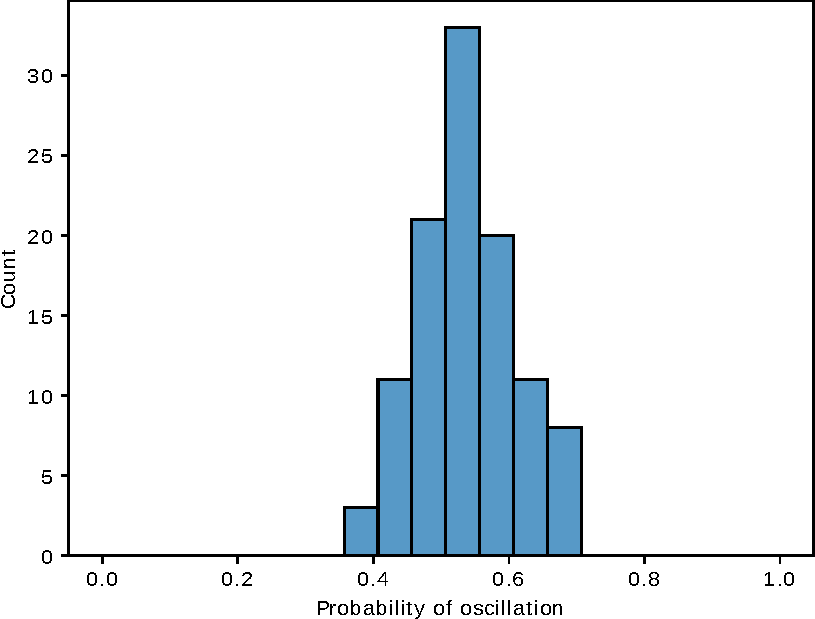
\includegraphics[width=\textwidth]{svm_scramble_2_edit.pdf}
   \caption{
   }
   \label{fig:analysis-svc-proba-histogram-scramble}
  \end{subfigure}

  \caption[
    Histogram of probabilities of whether a time series in the test data set is classified as oscillatory by the SVC, and as a control,
    with labels randomly re-assorted to time series.
  ]{
    \textbf{(\ref{fig:analysis-svc-proba-histogram-model})}
    Histogram of probabilities of whether a time series in the test data set is classified as oscillatory by the SVC (featurisation with \textit{catch22}, $\gamma = 1/22$, $C = 10$), and as a control
    \textbf{(\ref{fig:analysis-svc-proba-histogram-scramble})}
    with labels randomly reassigned.
  }
  \label{fig:analysis-svc-proba-histogram}
\end{figure}


\begin{figure}
  \centering
  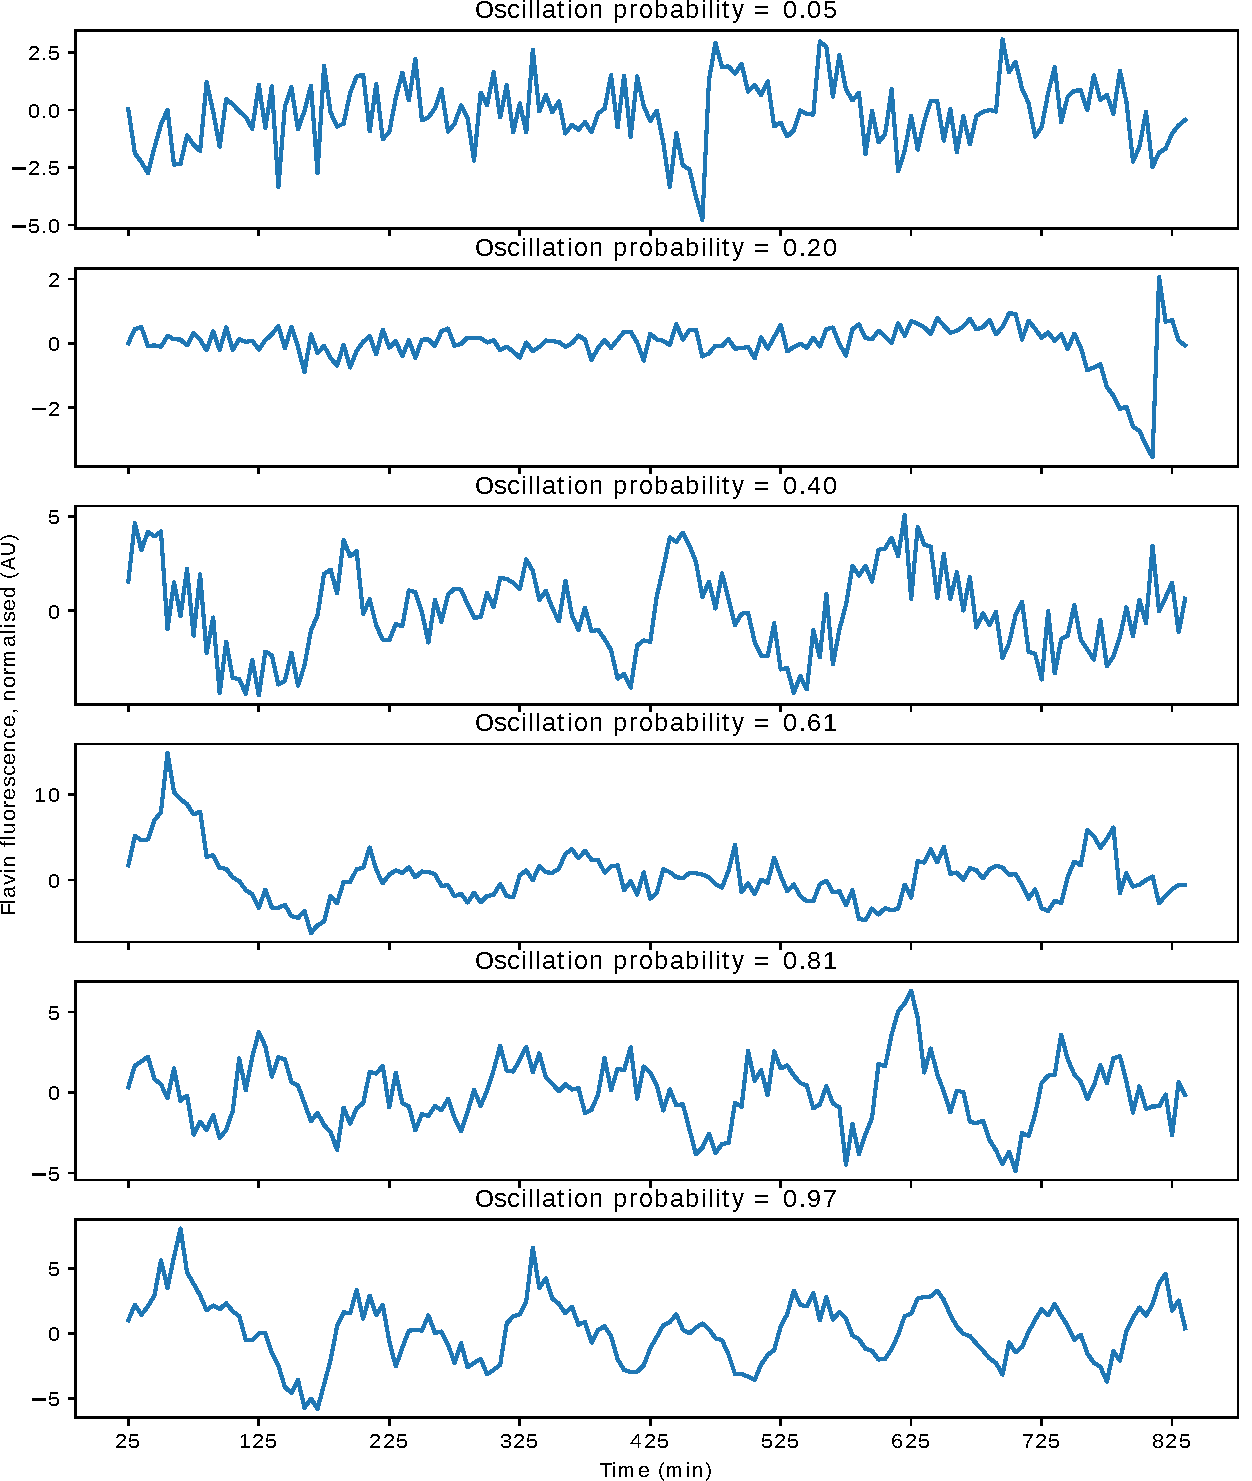
\includegraphics[width=0.8\textwidth]{svm_3_edit.pdf}

  \caption{
    Sample time series arranged by probability that each is oscillatory, as predicted by the support vector classifier.
  }
  \label{fig:analysis-svc-proba-gallery}
\end{figure}

To predict the probability that each time series was oscillatory, I used Platt scaling  \parencite{plattProbabilisticOutputsSupport1999} with the support vector classifier, as implemented by the \texttt{predict\_proba} method in the Python package \texttt{scikit\_learn}.
Platt scaling involves finding parameters for a logistic sigmoid function which approximates the posterior class probability for a binary classifier.
Fig.\ \ref{fig:analysis-svc-proba-histogram-model} suggests that the classifier performed well in discriminating between the two classes, as evidenced by the U-shaped histogram of probabilities, in contrast to the control (Fig.\ \ref{fig:analysis-svc-proba-histogram-scramble}).
In addition, Fig.\ \ref{fig:analysis-svc-proba-gallery} demonstrates that the probabilities can serve as a good score to rank time series by oscillation quality.


\section{Period estimation using the autocorrelation function}
\label{sec:analysis-characterisation}

Estimating the period of oscillatory time series is important as it provides a quantitative measure of how yeast metabolic cycles respond to genetic nutrient perturbations.
To show that the autocorrelation function can be used to estimate the period and noise properties of both symmetric and asymmetric oscillations, I adapted the autocorrelation function as used by \textcite{pietschDeterminingGrowthRates2023} (Methods Section~\ref{subsec:methods-computational-xcf}).
To calibrate the method, I generated synthetic oscillations --- sinusoids and the FitzHugh-Nagumo oscillator \parencite{fitzhughImpulsesPhysiologicalStates1961} --- to investigate the effect of their properties on the autocorrelation function.
Subsequently, I applied the autocorrelation function to characterise experimentally-recorded time series.
Details on how the sinusoids and the FitzHugh-Nagumo oscillators were defined can be found in Methods Section~\ref{subsec:methods-computational-synthetic}.

\subsection{Effect of noise parameters on the autocorrelation function of synthetic sinusoids}
\label{subsec:analysis-characterisation-acf-sinusoid}

\begin{figure}
  \centering
  \begin{subfigure}[t]{0.6\textwidth}
  \centering
    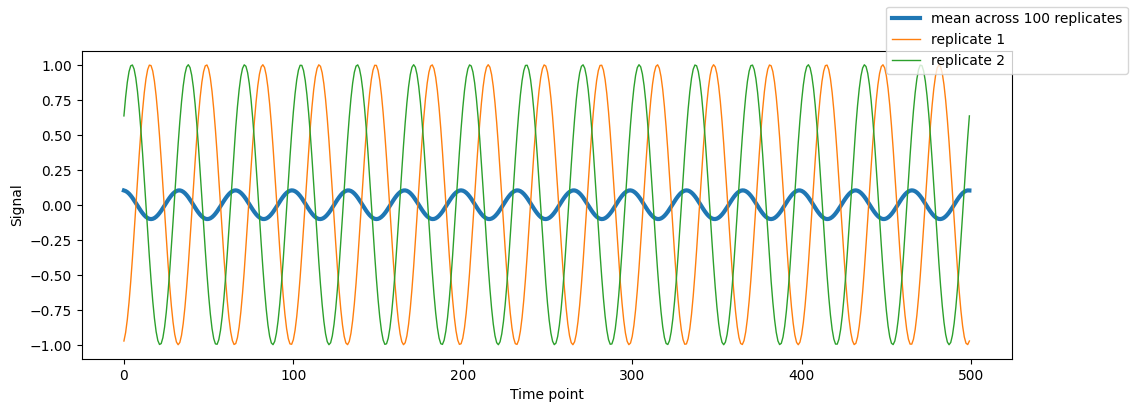
\includegraphics[width=\linewidth]{sinusoids_outofphase}
    \caption{
    }
    \label{fig:acf-sinusoids-nonoise-ts}
  \end{subfigure}%
  \centering
  \begin{subfigure}[t]{0.4\textwidth}
  \centering
    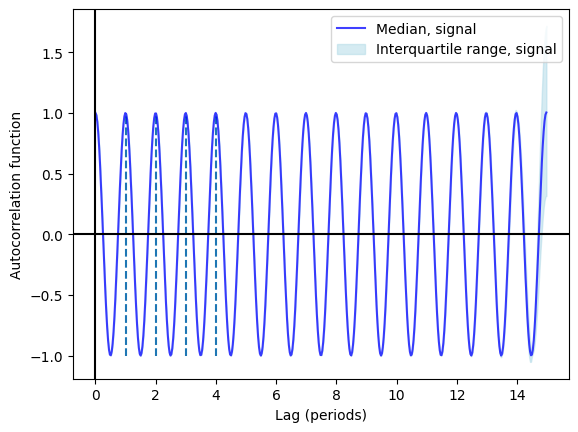
\includegraphics[width=\linewidth]{sinusoids_outofphase_acf_corrected}
    \caption{
    }
    \label{fig:acf-sinusoids-nonoise-acf}
  \end{subfigure}

  \begin{subfigure}[t]{0.6\textwidth}
  \centering
    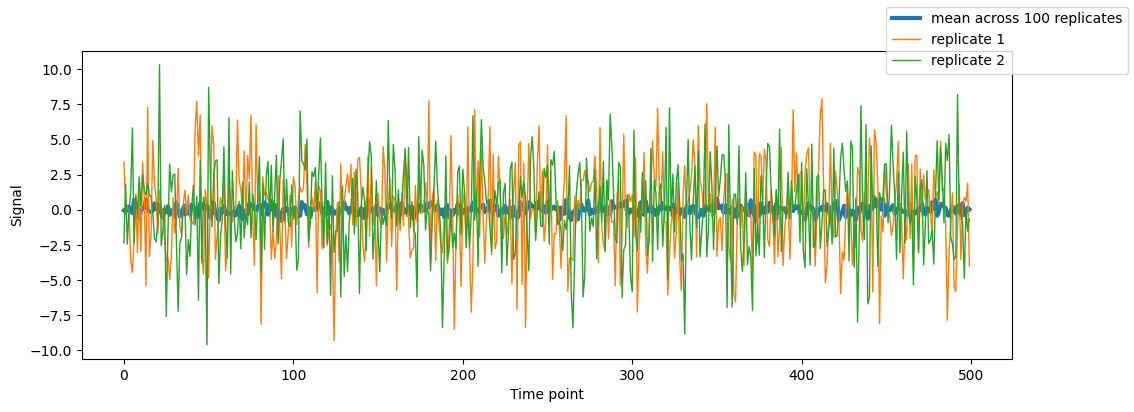
\includegraphics[width=\linewidth]{verynoisysinusoids_outofphase}
    \caption{
    }
    \label{fig:acf-sinusoids-gausnoise-ts}
  \end{subfigure}%
  \centering
  \begin{subfigure}[t]{0.4\textwidth}
  \centering
    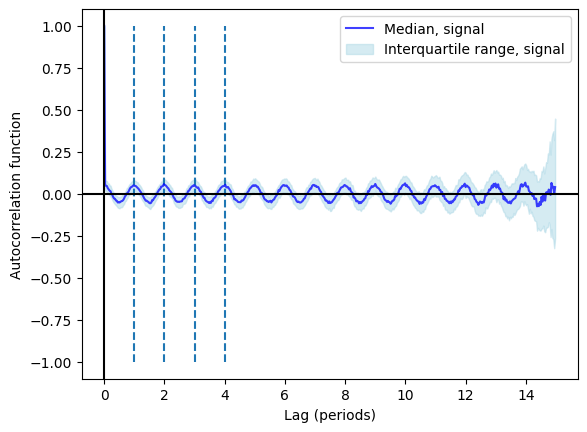
\includegraphics[width=\linewidth]{verynoisysinusoids_outofphase_acf}
    \caption{
    }
    \label{fig:acf-sinusoids-gausnoise-acf}
  \end{subfigure}

  \begin{subfigure}[t]{0.6\textwidth}
  \centering
    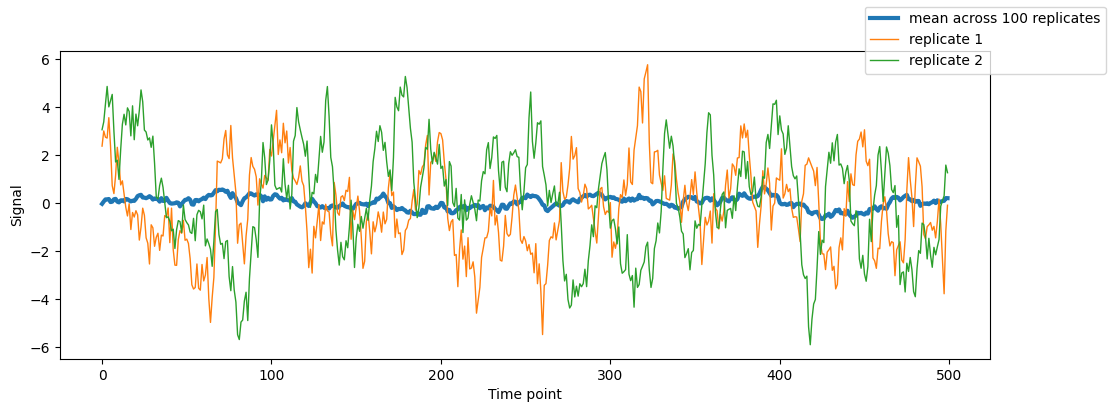
\includegraphics[width=\linewidth]{gillespie_k5_d0p05_mean}
    \caption{
    }
    \label{fig:acf-sinusoids-gillnoise-ts}
  \end{subfigure}%
  \centering
  \begin{subfigure}[t]{0.4\textwidth}
  \centering
    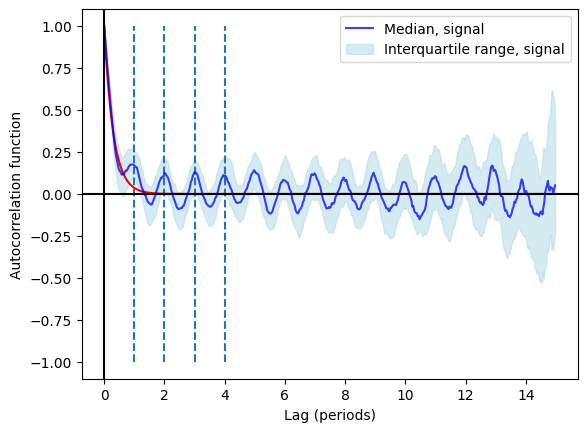
\includegraphics[width=\linewidth]{gillespie_k5_d0p05_acf}
    \caption{
    }
    \label{fig:acf-sinusoids-gillnoise-acf}
  \end{subfigure}

  \caption[
    Sample sinusoids without noise, with Gaussian noise, and with Gillespie noise, along with their autocorrelation functions.
  ]{
    %Effect of type of noise on the autocorrelation function.
    \textbf{(\ref{fig:acf-sinusoids-nonoise-ts})} Sample sinusoids without noise, and 
    \textbf{(\ref{fig:acf-sinusoids-nonoise-acf})} its autocorrelation function.
    %
    \textbf{(\ref{fig:acf-sinusoids-gausnoise-ts})} Sample sinusoids with Gaussian noise defined by drawing samples from $\mathcal{N}(0,\sigma^{2}=3)$, and 
    \textbf{(\ref{fig:acf-sinusoids-gausnoise-acf})} its autocorrelation function.
    %
    \textbf{(\ref{fig:acf-sinusoids-gillnoise-ts})} Sample sinusoids of with Gillespie noise ($k_{0} = 5$ and $d_{0} = 0.05$), and 
    \textbf{(\ref{fig:acf-sinusoids-gillnoise-acf})} its autocorrelation function.
    Red line is defined by $y = \me^{-2d_{0}T}$, where $T$ represents the lag in units of period of the sinusoids.
    %
    For each case, the frequency of the sinusoids was 0.03, and there were 100 repeats, randomly out-of-phase.
  }
  \label{fig:acf-sinusoids}
\end{figure}

To compare the effect of Gaussian noise and Gillespie noise on the autocorrelation function, I computed the autocorrelation functions from a population of sinusoids with either type of noise added via element-wise sums.

% [Show working -- i.e. the mathematical derivations that make me expect results?]
% [Equations -- clear lines before/after, rather than having them in-line?]

Fig.\ \ref{fig:acf-sinusoids-nonoise-acf} shows that the autocorrelation function computed from a population of out-of-phase sinusoids could be modelled by a cosine with the same period as the sinusoids.
Following this, Fig.\ \ref{fig:acf-sinusoids-gausnoise-acf} shows that the addition of Gaussian noise preserved the point $(0,1)$, but the amplitude of the cosine that models the autocorrelation function was decreased.
Furthermore, the variation of the autocorrelation function among time series at long lags was increased, as evidenced by the interquartile range, because less data was used to compute the autocorrelation function at longer lags.% (mathematical derivation in appendix ...).

Gillespie noise is based on the birth-death process, and its two parameters control noise parameters (Methods Section~\ref{subsec:methods-computational-synthetic}).
Specifically, given a birth rate $k_{0}$ and a death rate $d_{0}$, the noise has a standard deviation of noise amplitude $A = \sqrt{k_{0}/d_{0}}$ and noise timescale $\tau = 1/d_{0}$.
% [Show working -- i.e. the mathematical derivations that make me expect this exponential fit?]
% Though Peter said this `is not trivial'.
Fig.\ \ref{fig:acf-sinusoids-gillnoise-acf} shows that when Gillespie noise was added to the sinusoids, the medium autocorrelation followed the exponential decay function $y = \me^{-2d_{0}T}$, where $T$ represents lag.
In addition, the locations of the peaks of the autocorrelation function were preserved.
The observation thus suggests that the death rate $d_{0}$ parameter of Gillespie noise controlled the shape of the autocorrelation function.


\begin{figure}
  \centering
  \begin{subfigure}[t]{0.6\textwidth}
  \centering
    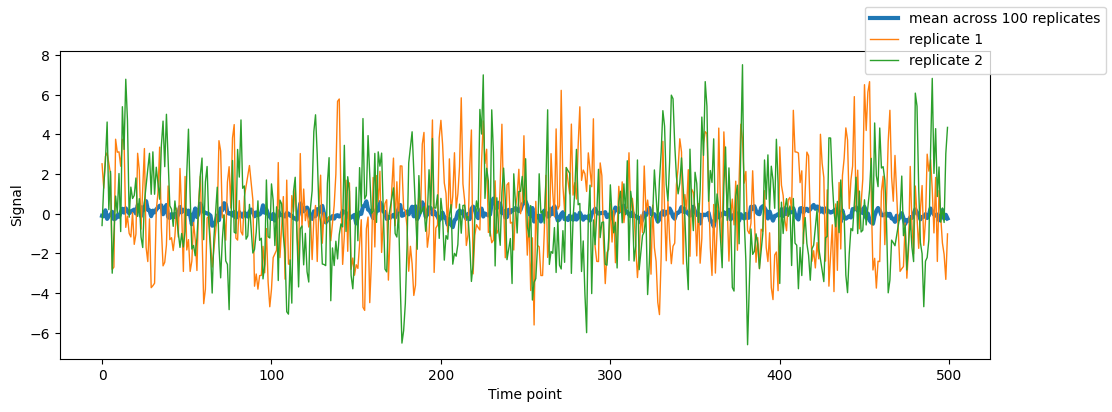
\includegraphics[width=\linewidth]{gillespie_k5_d0p5_mean.png}
    \caption{
    }
    \label{fig:acf-noisetimescale-highd0-ts}
  \end{subfigure}%
  \begin{subfigure}[t]{0.4\textwidth}
  \centering
    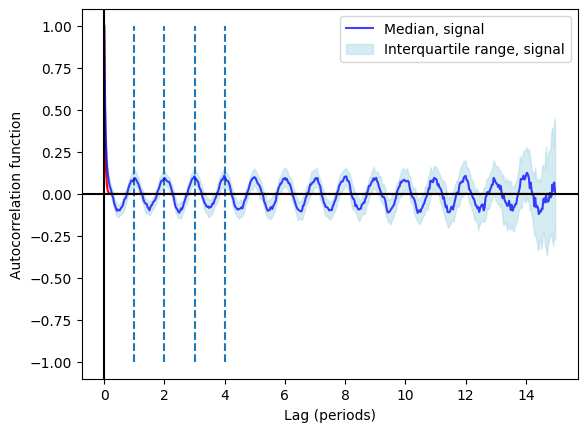
\includegraphics[width=\linewidth]{gillespie_k5_d0p5_acf.png}
    \caption{
    }
    \label{fig:acf-noisetimescale-highd0-acf}
  \end{subfigure}

  \begin{subfigure}[t]{0.6\textwidth}
  \centering
    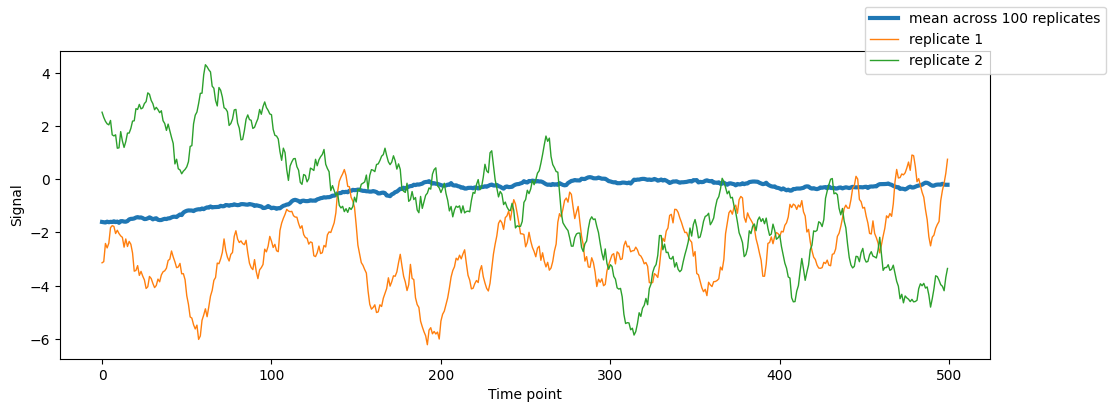
\includegraphics[width=\linewidth]{gillespie_k5_d0p005_mean.png}
    \caption{
    }
    \label{fig:acf-noisetimescale-lowd0-ts}
  \end{subfigure}%
  \begin{subfigure}[t]{0.4\textwidth}
  \centering
    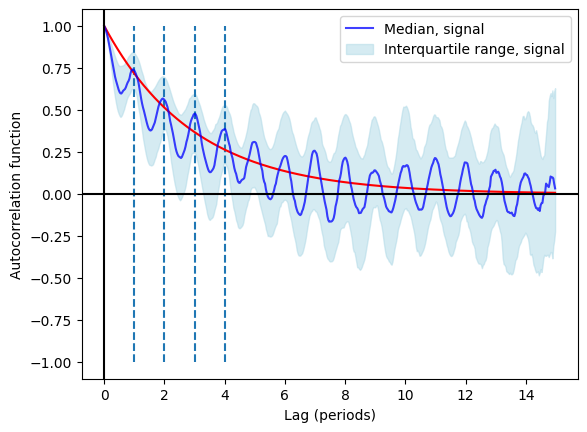
\includegraphics[width=\linewidth]{gillespie_k5_d0p005_acf.png}
    \caption{
    }
    \label{fig:acf-noisetimescale-lowd0-acf}
  \end{subfigure}

  \caption[
    Effect of death rate of Gillespie noise on the autocorrelation function.
  ]{
    %Effect of death rate ($d_{0}$) of Gillespie noise on the autocorrelation function.
    \textbf{(\ref{fig:acf-noisetimescale-highd0-ts})} Sample sinusoids with Gillespie noise ($k_{0} = 5$ and $d_{0} = 0.5$), and 
    \textbf{(\ref{fig:acf-noisetimescale-highd0-acf})} its autocorrelation function.
    %
    \textbf{(\ref{fig:acf-noisetimescale-lowd0-ts})} Sample sinusoids with Gillespie noise ($k_{0} = 5$ and $d_{0} = 0.005$), and 
    \textbf{(\ref{fig:acf-noisetimescale-lowd0-acf})} its autocorrelation function.
    %
    Red lines are defined by $y = \me^{-2d_{0}T}$, where $T$ represents the lag in units of period of the sinusoids.
    %
    For each case, the frequency of the sinusoids was 0.03, and there were 100 repeats, randomly out-of-phase.
  }
  \label{fig:acf-noisetimescale}
\end{figure}


% \begin{figure}
%   \centering
%   \begin{subfigure}[t]{0.5\textwidth}
%   \centering
%     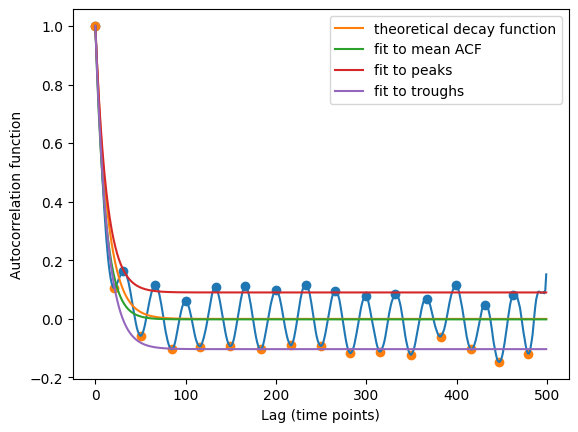
\includegraphics[width=\linewidth]{acf_fit_example.png}
%     \caption{
%     }
%     \label{fig:acf-noisetimescale-effect-fit}
%   \end{subfigure}%
%   \begin{subfigure}[t]{0.5\textwidth}
%   \centering
%     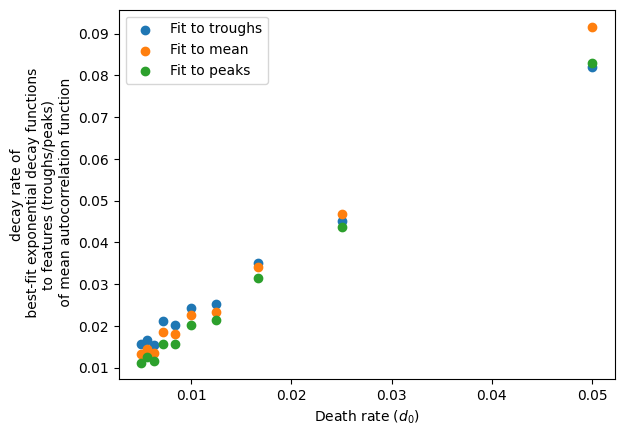
\includegraphics[width=\linewidth]{deathrate_vs_decay.png}
%     \caption{
%     }
%     \label{fig:acf-noisetimescale-effect-relationship}
%   \end{subfigure}

%   \caption[
%     Fitting exponential decay functions to estimate $d_{0}$ from the autocorrelation function.
%   ]{
%     \textbf{(\ref{fig:acf-noisetimescale-effect-fit})} Fitting exponential decay functions to estimate $d_{0}$ from the autocorrelation function.
%     \textbf{(\ref{fig:acf-noisetimescale-effect-relationship})} The relationship between $d_{0}$ and the decay rate $D$ found from fitting exponential decay functions to the mean autocorrelation function, the peaks, and the troughs of this mean function.
%     Here, $k_{0}$ was held constant at 5.
%   }
%   \label{fig:acf-noisetimescale-effect}
% \end{figure}

To quantify the effect of the noise timescale on the shape of the autocorrelation function, I varied the death rate parameter $d_{0}$ when generating Gillespie noise.
%
Fig.\ \ref{fig:acf-noisetimescale} shows that a higher death rate decreased the decay timescale of the autocorrelation function (Fig.\ \ref{fig:acf-noisetimescale-highd0-acf}), while a lower death rate introduced long-term trends in the simulated signals (Fig.\ \ref{fig:acf-noisetimescale-lowd0-ts}).
A lower death rate also increased the variation between autocorrelation functions between replicates (Fig.\ \ref{fig:acf-noisetimescale-lowd0-acf}).

% To show how $d_{0}$ can be estimated from the autocorrelation function, I fitted exponential decay functions to the mean autocorrelation, the peaks of the mean function, and the troughs of the mean functions using non-linear least squares fitting (Fig.\ \ref{fig:acf-noisetimescale-effect-fit}).
% The functions were of the form:

% \begin{equation}
%   y = (1-C)\me^{-DT}+C
%   \label{eq:acf-expofit}
% \end{equation}

% where $y$ represents the vertical axis (autocorrelation axis), $T$ represents the lag multiples of the period of the sinusoid oscillator, and with $C$ and $D$ being variable parameters whose values are to be determined.

% Fig.\ \ref{fig:acf-noisetimescale-effect-relationship} suggests that the decay rates $D$ of the autocorrelation function increases linearly with $d_{0}$.
% In other words, the death rate $d_{0}$ controls the decay rate $D$ of the autocorrelation function.
% Conversely, if $D$ can be estimated from the autocorrelation function, then the noise timescale of the time series can be estimated.


\begin{figure}
  \centering
  \begin{subfigure}[t]{0.6\textwidth}
  \centering
    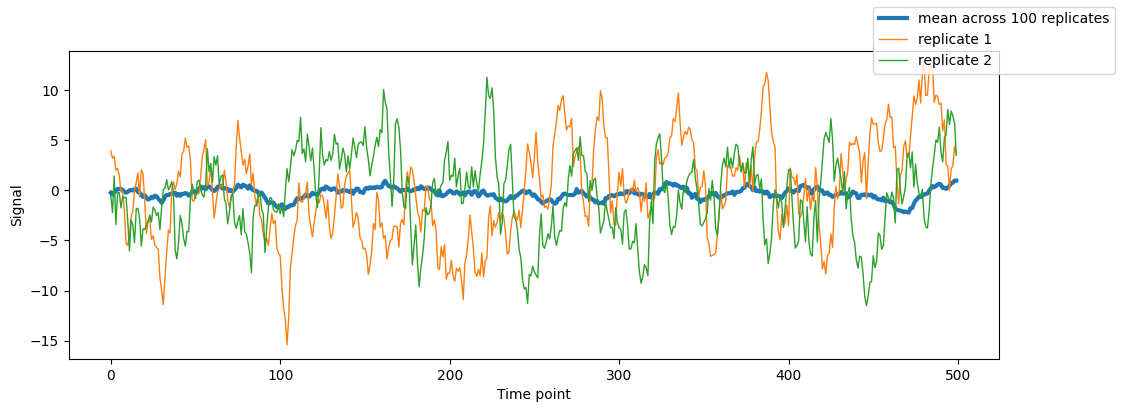
\includegraphics[width=\linewidth]{gillespie_k25_d0p05_mean.png}
    \caption{
    }
    \label{fig:acf-noiseamplitude-highk0-ts}
  \end{subfigure}%
  \begin{subfigure}[t]{0.4\textwidth}
  \centering
    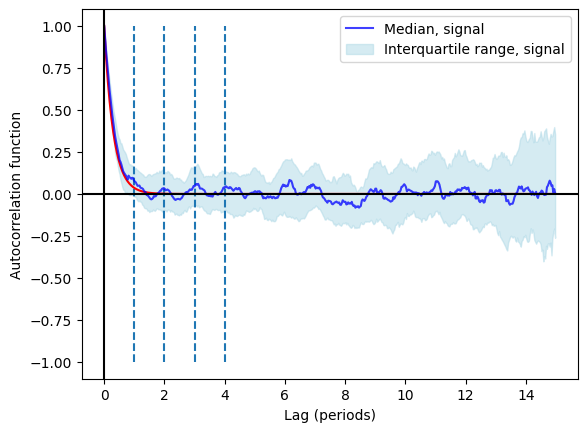
\includegraphics[width=\linewidth]{gillespie_k25_d0p05_acf.png}
    \caption{
    }
    \label{fig:acf-noiseamplitude-highk0-acf}
  \end{subfigure}

  \begin{subfigure}[t]{0.6\textwidth}
  \centering
    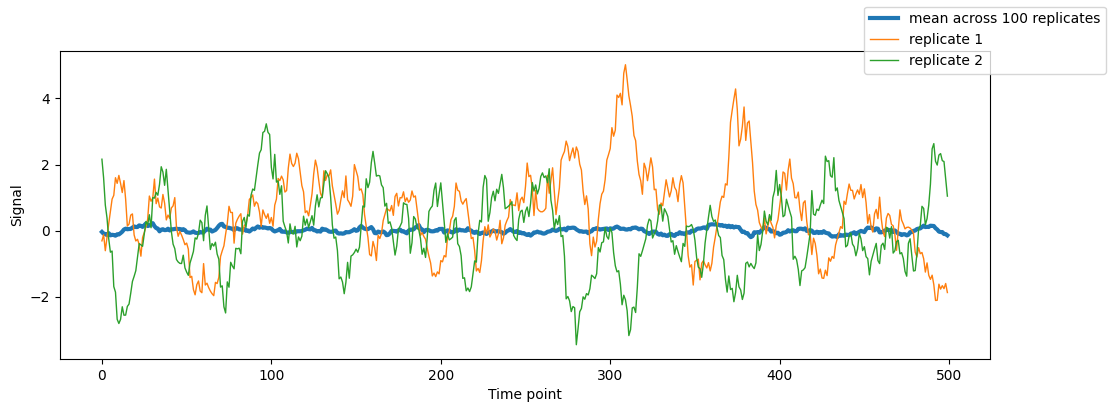
\includegraphics[width=\linewidth]{gillespie_k1_d0p05_mean.png}
    \caption{
    }
    \label{fig:acf-noiseamplitude-lowk0-ts}
  \end{subfigure}%
  \begin{subfigure}[t]{0.4\textwidth}
  \centering
    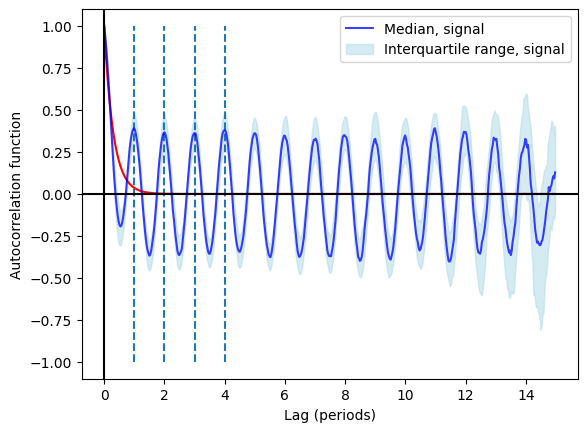
\includegraphics[width=\linewidth]{gillespie_k1_d0p05_acf.png}
    \caption{
    }
    \label{fig:acf-noiseamplitude-lowk0-acf}
  \end{subfigure}

  \caption[
    Effect of birth rate of Gillespie noise on the autocorrelation function.
  ]{
    %Effect of birth rate ($k_{0}$) of Gillespie noise on the autocorrelation function.
    \textbf{(\ref{fig:acf-noiseamplitude-highk0-ts})} Sample sinusoids with Gillespie noise ($k_{0} = 25$ and $d_{0} = 0.05$), and 
    \textbf{(\ref{fig:acf-noiseamplitude-highk0-acf})} its autocorrelation function.
    %
    \textbf{(\ref{fig:acf-noiseamplitude-lowk0-ts})} Sample sinusoids with Gillespie noise ($k_{0} = 1$ and $d_{0} = 0.05$), and 
    \textbf{(\ref{fig:acf-noiseamplitude-lowk0-acf})} its autocorrelation function.
    %
    Red lines are defined by $y = \me^{-2d_{0}T}$, where $T$ represents the lag in units of period of the sinusoids.
    %
    For each case, the frequency of the sinusoids was 0.03, and there were 100 repeats, randomly out-of-phase.
  }
  \label{fig:acf-noiseamplitude}
\end{figure}


% \begin{figure}
%   \centering
%   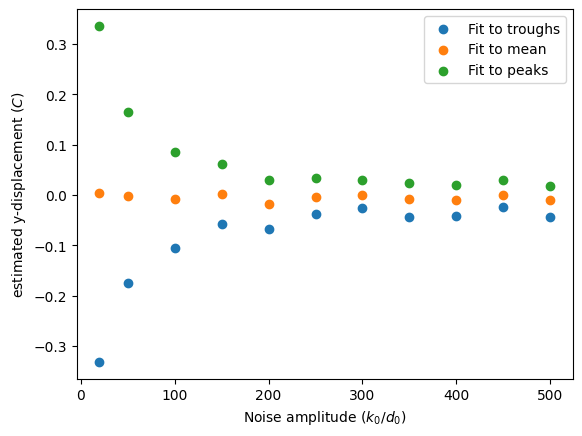
\includegraphics[width=0.6\linewidth]{birthrate_vs_ydispl.png}
%   \caption[
%     The relationship between the noise amplitude and the $y$-displacement $C$ found from fitting exponential decay functions to the mean autocorrelation function.
%   ]{
%     The relationship between the noise amplitude and the $y$-displacement $C$ found from fitting exponential decay functions to the mean autocorrelation function, the peaks, and the troughs of this mean function.
%     Here, $d_{0}$ was held constant at 0.05.
%   }
%   \label{fig:acf-noiseamplitude-effect}
% \end{figure}


To quantify the effect of the noise amplitude on the autocorrelation function, I varied the birth rate parameter $k_{0}$ when generating Gillespie noise.
Fig.\ \ref{fig:acf-noiseamplitude} shows that a higher birth rate increased the amplitude of noise (Fig.\ \ref{fig:acf-noiseamplitude-highk0-ts}) and increased the variation between replicate autocorrelation functions (Fig.\ \ref{fig:acf-noiseamplitude-highk0-acf}), while the opposite was true for a higher birth rate (Figs.\ \ref{fig:acf-noiseamplitude-lowk0-ts}--\ref{fig:acf-noiseamplitude-lowk0-acf}).

% To show how the noise amplitude can be estimated from the autocorrelation function, I fit exponential decay functions (Eq.\ \ref{eq:acf-expofit}) as in Fig.\ \ref{fig:acf-noisetimescale-effect-fit}.
% Fig.\ \ref{fig:acf-noiseamplitude-effect} suggests that the $y$-displacements $C$ of the exponential fits to peaks and troughs converged to 0 as $k_{0}/d_{0}$ increased, showing that the amplitude of the oscillations in the autocorrelation function decreases as the noise amplitude increases.
% In other words, the birth rate $d_{0}$ controls the $y$-displacement parameter $C$ of the autocorrelation function, which is a proxy for the function's amplitude.
% Conversely, if $C$ can be estimated from the autocorrelation function, then the noise amplitude of the time series can be estimated.


\subsection{FitzHugh-Nagumo oscillator: effect of oscillation shape}
\label{subsec:analysis-characterisation-acf-fhn}

\begin{figure}
  \centering
  \begin{subfigure}[t]{0.6\textwidth}
  \centering
    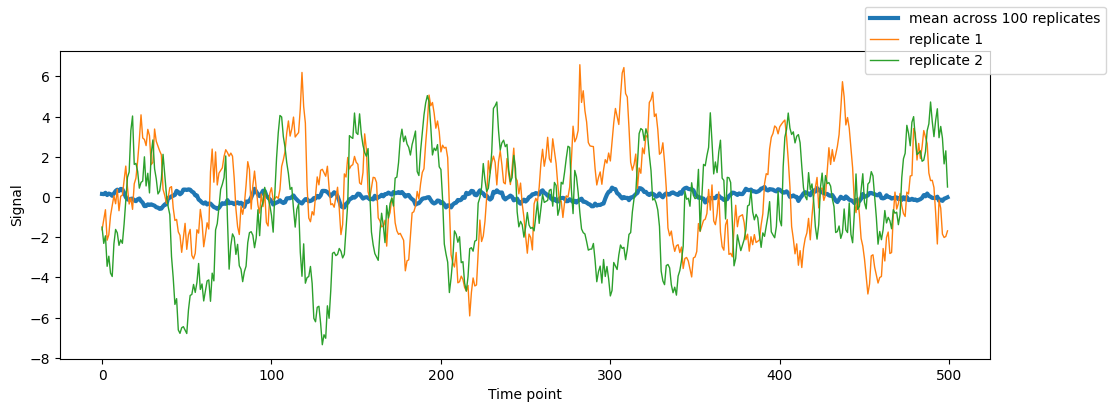
\includegraphics[width=\linewidth]{fhn_meanplot}
    \caption{
    }
    \label{fig:acf-fhn-gillnoise-ts}
  \end{subfigure}%
  \begin{subfigure}[t]{0.4\textwidth}
  \centering
    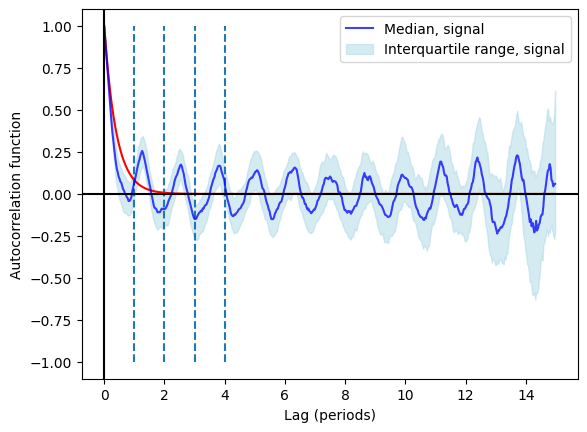
\includegraphics[width=\linewidth]{fhn_acf}
    \caption{
    }
    \label{fig:acf-fhn-gillnoise-acf}
  \end{subfigure}

  \caption[
    Sample FitzHugh-Nagumo oscillators with Gillespie noise, and
    its autocorrelation function.
  ]{
    %The autocorrelation function of FitzHugh-Nagumo oscillators with Gillespie noise.
    \textbf{(\ref{fig:acf-fhn-gillnoise-ts})} Sample FitzHugh-Nagumo oscillators ($RI_{\mathrm{ext}}$ = 0.4, $\tau$ = 12.5, $a$ = 0.7, $b$ = 0.82) with Gillespie noise ($k_{0} = 5$ and $d_{0} = 0.05$), and 
    \textbf{(\ref{fig:acf-fhn-gillnoise-acf})} its autocorrelation function.
    Red line is defined by $y = \me^{-2d_{0}T}$, where $T$ represents the lag in units of period of the sinusoids.
    %
    There were 100 repeats, randomly out-of-phase.
  }
  \label{fig:acf-fhn}
\end{figure}


% \begin{figure}
%   \centering
%   \begin{subfigure}[t]{0.45\textwidth}
%   \centering
%     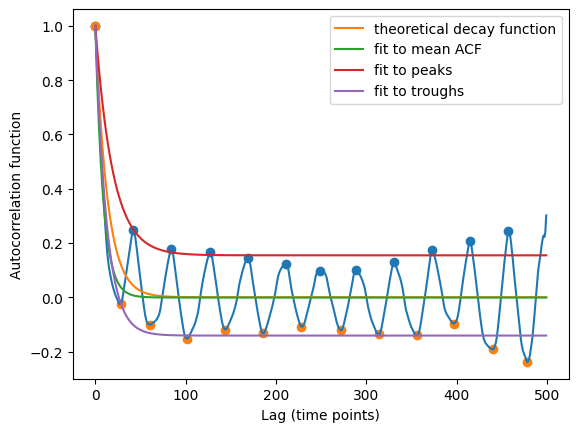
\includegraphics[width=\linewidth]{fhn_expofit}
%     \caption{
%     }
%     \label{fig:acf-fhn-noiseparams-fit}
%   \end{subfigure}%
%   \begin{subfigure}[t]{0.45\textwidth}
%   \centering
%     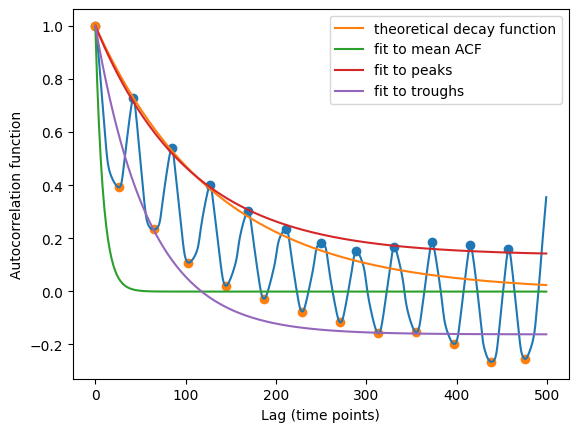
\includegraphics[width=\linewidth]{fhn_highnts_expofit}
%     \caption{
%     }
%     \label{fig:acf-fhn-noiseparams-fit-highnts}
%   \end{subfigure}
%
%   \begin{subfigure}[t]{0.45\textwidth}
%   \centering
%     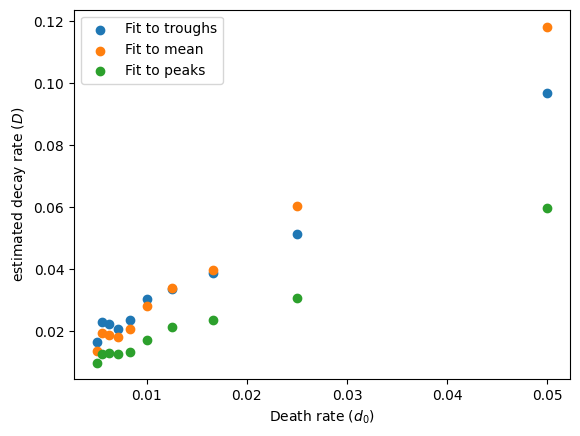
\includegraphics[width=\linewidth]{fhn_deathrate_vs_decay.png}
%     \caption{
%     }
%     \label{fig:acf-fhn-noiseparams-noisetimescale}
%   \end{subfigure}%
%   \begin{subfigure}[t]{0.45\textwidth}
%   \centering
%     \includegraphics[width=\linewidth]{fhn_birthrate_vs_ydispl.png}
%     \caption{
%     }
%     \label{fig:acf-fhn-noiseparams-noiseamplitude}
%   \end{subfigure}

%   \caption[
%     Effect of Gillespie noise parameters on the autocorrelation function of FitzHugh-Nagumo oscillators.
%   ]{
%     \textbf{(\ref{fig:acf-fhn-noiseparams-fit})}
%     Fitting exponential decay functions of the form $y = (1-C)\me^{-DT}+C$, with $C$ and $D$ as variable parameters, to the autocorrelation function, generated with $k_{0}=5$ and $d_{0}=0.05$, and
%     \textbf{(\ref{fig:acf-fhn-noiseparams-fit-highnts})}
%     with $k_{0}=5$ and $d_{0}=0.005$.
%     \textbf{(\ref{fig:acf-fhn-noiseparams-noisetimescale})}
%     The relationship between $d_{0}$ and the decay rate $D$ ($k_{0}=5$).
%     \textbf{(\ref{fig:acf-fhn-noiseparams-noiseamplitude})}
%     The relationship between $k_{0}/d_{0}$ and $y$-displacement $C$ of the exponential fit ($d_{0}=0.05$)
%   }
%   \label{fig:acf-fhn-noiseparams}
% \end{figure}

To test whether Gillespie noise parameters can be estimated from the autocorrelation function computed from an asymmetric oscillation, I repeated the exponential fitting in section~\ref{subsec:analysis-characterisation-acf-sinusoid} on the FitzHugh-Nagumo oscillator as defined in the Methods (Section~\ref{subsec:methods-computational-synthetic}).

Fig.\ \ref{fig:acf-fhn-gillnoise-acf} shows that when the oscillator had a different shape, the waves in the autocorrelation function changed shape, becoming more pointed.
% In addition, Fig.\ \ref{fig:acf-fhn-noiseparams-fit-highnts} suggests that fitting an exponential decay function to the autocorrelation function to estimate noise parameters was less reliable, particularly with high noise timescales.
% As a consequence, estimating the noise timescale $\tau$ from the decay rate $D$ of the exponential decay function produced a greater range of uncertainty (Fig.\ \ref{fig:acf-fhn-noiseparams-noisetimescale}).
% However, estimating the noise amplitude $A$ based on the y-displacement $C$ of the exponential decay function remained as reliable as the sinusoid oscillator case (Fig.\ \ref{fig:acf-fhn-noiseparams-noiseamplitude}).


\subsection{Real data}
\label{subsubsec:analysis-characterisation-real}

\begin{figure}
  \centering
  \begin{subfigure}[t]{0.8\textwidth}
  \centering
    \includegraphics[width=\linewidth]{acf_sinusoid_biol_ts.png}
    \caption{
    }
    \label{fig:acf-sinusoid-biol-ts}
  \end{subfigure}

  \begin{subfigure}[t]{0.5\textwidth}
  \centering
    \includegraphics[width=\linewidth]{acf_sinusoid_biol_acf.png}
    \caption{
    }
    \label{fig:acf-sinusoid-biol-acf}
  \end{subfigure}

  % \begin{subfigure}[t]{0.5\textwidth}
  % \centering
  %   \includegraphics[width=\linewidth]{acf_sinusoid_biol_acf_fit.png}
  %   \caption{
  %   }
  %   \label{fig:acf-sinusoid-biol-acf-fit}
  % \end{subfigure}

  \caption[
    Sample time series of flavin autofluorescence, its autocorrelation function, and fitting exponential decay functions.
  ]{
    \textbf{(\ref{fig:acf-sinusoid-biol-ts})}
    Sample time series of flavin autofluorescence.
    \textbf{(\ref{fig:acf-sinusoid-biol-acf})}
    Autocorrelation function across a population of time series of flavin autofluorescence.
    % \textbf{(\ref{fig:acf-sinusoid-biol-acf-fit})}
    % Fitting exponential decay functions to determine noise parameters, lag axis scaled to match Fig.\ \ref{fig:acf-noisetimescale-effect}.
  }
  \label{fig:acf-sinusoid-biol}
\end{figure}

To deduce the period and noise parameters of a experimentally-recorded sinusoid-like signal (Fig.\ \ref{fig:acf-sinusoid-biol-ts}), I computed the autocorrelation functions of a population of flavin autofluorescence time series (Fig.\ \ref{fig:acf-sinusoid-biol-acf}).
% , and fitted exponential functions to the mean autocorrelation function, scaled to have amplitudes and periods fit the simulated sinusoids (Fig.\ \ref{fig:acf-sinusoid-biol-acf-fit}).
The autocorrelation function suggests an average period of 19 time points, corresponding to \SI{95}{\minute}, as expected from the nutrient conditions.
However, estimation of noise parameters was complicated by the damping in the autocorrelation function, giving a different shape compared to the synthetic data and fewer peaks and troughs for fitting.
Nevertheless, the decay rate $D$ of the exponential function fitted to the mean autocorrelation function suggested a noise timescale of 7.16 and the y-displacement $C$ of the exponential function fitted to the peaks of the autocorrelation function suggested a noise amplitude of 161.84.


\begin{figure}
  \centering
  \begin{subfigure}[t]{0.8\textwidth}
  \centering
    \includegraphics[width=\linewidth]{acf_fhn_biol_ts.png}
    \caption{
    }
    \label{fig:acf-fhn-biol-ts}
  \end{subfigure}

  \begin{subfigure}[t]{0.5\textwidth}
  \centering
    \includegraphics[width=\linewidth]{acf_fhn_biol_acf.png}
    \caption{
    }
    \label{fig:acf-fhn-biol-acf}
  \end{subfigure}

  % \begin{subfigure}[t]{0.5\textwidth}
  % \centering
  %   \includegraphics[width=\linewidth]{acf_fhn_biol_acf_fit.png}
  %   \caption{
  %   }
  %   \label{fig:acf-fhn-biol-acf-fit}
  % \end{subfigure}

  \caption[
    Sample time series of histone 2B abundance, its autocorrelation function, and fitting exponential decay functions.
  ]{
    \textbf{(\ref{fig:acf-fhn-biol-ts})}
    Sample time series of histone 2B abundance.
    \textbf{(\ref{fig:acf-fhn-biol-acf})}
    Autocorrelation function across a population of time series of histone 2B abundance.
    % \textbf{(\ref{fig:acf-fhn-biol-acf-fit})}
    % Fitting exponential decay functions to determine noise parameters.
  }
  \label{fig:acf-fhn-biol}
\end{figure}

In addition to flavin autofluorescence, I also recorded time series of histone 2B abundance as an indicator of the phases of the cell division cycle \parencite{garmendia-torresMultipleInputsEnsure2018}, to investigate whether the flavin autofluorescence oscillations and the cell division cycle synchronised.
The abundance of histone 2B follow an asymmetric oscillation (Fig.\ \ref{fig:acf-fhn-biol-ts}).

Similar to the previous section, to deduce the period and noise parameters of this signal, I computed the autocorrelation functions of a population of histone 2B abundance time series (Fig.\ \ref{fig:acf-fhn-biol-acf}).
% , and fitted exponential functions to the mean autocorrelation function, scaled to have amplitudes and periods fit the simulated FitzHugh-Nagumo oscillators (Fig.\ \ref{fig:acf-fhn-biol-acf-fit}).
The autocorrelation function also suggests an average period of 19 time points, corresponding to \SI{95}{\minute}.
As was the case for the flavin autofluorescence time series, the damping in the autocorrelation function complicated estimation of noise parameters; though the decay rate $D$ of the exponential function fitted to the mean autocorrelation function suggested a noise timescale of 11.19 and the y-displacement $C$ of the exponential function fitted to the peaks of the autocorrelation function suggested a noise amplitude of 292.41.
The differences of these noise parameters relative to the flavin autofluorescence time series suggest different noise properties, which can be explained by the different fluorescence channels and exposure times used to generate each type of signal.


\section{Detection of synchrony}
\label{sec:analysis-correlation}

To test a method to detect the synchrony and quantify the temporal lag between two types of oscillations, I computed the cross-correlation functions of a population of sinusoid and FitzHugh-Nagumo oscillators.
Cross-correlation has been used to investigate the relationship between the expression levels of two genes in a model feed-forward loop \parencite{dunlopRegulatoryActivityRevealed2008},
and to investigate the relationship between instantaneous growth rate and the expression of \textit{lac} genes of enzymes in central metabolism across a population of \textit{E. coli} cells \parencite{kivietStochasticityMetabolismGrowth2014}.

\subsection{Synthetic data}
\label{subsubsec:analysis-correlation-synthetic}

\begin{figure}
  \centering
  \begin{subfigure}[t]{0.6\textwidth}
  \centering
    \includegraphics[width=\linewidth]{sinusoid_and_fitzhughnagumo_nonoise.png}
    \caption{
    }
    \label{fig:xcf-nonoise-ts}
  \end{subfigure}%
  \centering
  \begin{subfigure}[t]{0.4\textwidth}
  \centering
    \includegraphics[width=\linewidth]{randomshift_sinusoid_fitzhughnagumo_xcf.png}
    \caption{
    }
    \label{fig:xcf-nonoise-xcf}
  \end{subfigure}

  \begin{subfigure}[t]{0.6\textwidth}
  \centering
    \includegraphics[width=\linewidth]{sinusoid_and_fitzhughnagumo_gillnoise.png}
    \caption{
    }
    \label{fig:xcf-gillnoise-ts}
  \end{subfigure}%
  \centering
  \begin{subfigure}[t]{0.4\textwidth}
  \centering
    \includegraphics[width=\linewidth]{randomshift_sinusoid_fitzhughnagumo_gillnoise_xcf.png}
    \caption{
    }
    \label{fig:xcf-gillnoise-xcf}
  \end{subfigure}

  \caption[
    Sample sinusoid and FitzHugh-Nagumo oscillators without noise and with Gillespie noise, along with their cross-correlation functions.
  ]{
    %Using the cross-correlation function to evaluate the shift of one synthetic time series relative to another with a different shape.
    \textbf{(\ref{fig:xcf-nonoise-ts})}
    (Blue) Sample sinusoid ($f = 0.0235$) and (orange) FitzHugh-Nagumo oscillator ($RI_{\mathrm{ext}}$ = 0.4, $\tau$ = 12.5, $a$ = 0.7, $b$ = 0.82) of the same frequency and without noise, and
    \textbf{(\ref{fig:xcf-nonoise-xcf})}
    the cross-correlation function of the FitzHugh-Nagumo oscillators with respect to the sinusoids.
    %
    \textbf{(\ref{fig:xcf-gillnoise-ts})}
    (Blue) Sample sinusoid and (orange) FitzHugh-Nagumo oscillator with same parameters as \ref{fig:xcf-nonoise-ts}, but with Gillespie noise ($d_{0} = 0.05$, $k_{0} = 5$), and
    \textbf{(\ref{fig:xcf-gillnoise-xcf})}
    the cross-correlation function of the FitzHugh-Nagumo oscillators with respect to the sinusoids.
    %
    For each case, there were 400 repeats, randomly out-of-phase.
  }
  \label{fig:xcf}
\end{figure}

Fig.\ \ref{fig:xcf-nonoise-xcf} shows that the cross-correlation function identifies that the sinusoids, on average, peaked 20 time points before the FitzHugh-Nagumo oscillators, close to the actual value of 20.75 time points.
This shift was evidenced by the position of the peak of the cross-correlation function closest to the vertical axis.
The cross-correlation function further showed that synchrony between the two oscillators was maintained along the entire time series, across all time series.
Furthermore, Fig.\ \ref{fig:xcf-gillnoise-xcf} suggests that even with strong Gillespie noise, the lag between the two oscillators could still be deduced from the cross-correlation function.


\subsection{Real data}
\label{subsubsec:analysis-correlation-real}

To show how the cross-correlation function can be used to quantify the synchrony between flavin autofluorescence oscillations and HTB2::mCherry levels in a population of cells, Fig.\ \ref{fig:xcf-biol} displays a sample pair of time series (Fig.\ \ref{fig:xcf-biol-ts}) and the cross-correlation function from the population of cells (Fig.\ \ref{fig:xcf-biol-xcf}).
The cross-correlation function suggests that the histone 2B oscillations peaked after the flavin autofluorescence oscillations by an average of \SI{5}{\minute}.

\begin{figure}
  \centering
  \begin{subfigure}[t]{1.0\textwidth}
  \centering
    \includegraphics[width=\linewidth]{single_birth_plot_nostar.pdf}
    \caption{
    }
    \label{fig:xcf-biol-ts}
  \end{subfigure}

  \begin{subfigure}[t]{0.7\textwidth}
  \centering
    \includegraphics[width=\linewidth]{xcf_edit.pdf}
    \caption{
    }
    \label{fig:xcf-biol-xcf}
  \end{subfigure}

  \caption[
    Sample time series of flavin autofluorescence and histone 2B abundance, along with the cross-correlation function.
  ]{
    \textbf{(\ref{fig:xcf-biol-ts})}
    Sample time series of flavin autofluorescence (blue) and histone 2B abundance (orange).
    \textbf{(\ref{fig:xcf-biol-xcf})}
    Cross-correlation function between the flavin autofluorescence time series and the histone 2B abundance time series.
  }
  \label{fig:xcf-biol}
\end{figure}


\section{Discussion}
\label{sec:analysis-discussion}

This chapter discusses methods to filter long-term trends in time series data, to visualise structures within a dataset of time series, to detect rhythmicity in a time series, to estimate period and noise parameters, and to detect the synchrony between two time series.

My results suggest that using a high-pass Butterworth filter to filter out long-term trends in time series data gives better control over the frequency profile of the time series than moving-average methods, which is often used to detrend time series from biological oscillators.
Such results highlight that a degree of caution is needed to choose methods for a crucial step in data analysis.

My exploration of UMAP and modularity clustering suggests that both methods were useful to discovering structure within time series, particularly in discriminating between oscillatory and non-oscillatory time series.
These methods further indicated sub-groups of time series that may have similar properties, such as shape or oscillation quality, which may correspond to sub-populations of metabolic cycle-producing cells in a culture.
The consistency between the two methods strongly suggest that such groups in the dataset are meaningful.

Subsequently, my exploration of three approaches to detect rhythmicity --- deriving a statistical test of a power spectrum, deriving a periodogram from an autoregressive model, and a binary classifier --- highlights the difficulty of rhythmicity detection in noisy biological time series.
The spectral method described by \parencite{glynnDetectingPeriodicPatterns2006a} had a modest performance.
The autoregressive model was able to identify the most likely period in some time series, but otherwise classified most time series as non-oscillatory, and lacked a tuning parameter.
Finally, the support vector classifier suggests that a simple machine learning model could be adapted for rhythmicity detection, subject to a good feature set and training data.

Ultimately, rhythmicity detection requires supplying a threshold in some form, be it a range of frequencies in which oscillations are expected \parencite{zielinskiStrengthsLimitationsPeriod2014}, a parameter that controls the proportion of time series detected as oscillatory, or training labels.
This is because there is no way to objectively specify a failure rate for a rhythmicity detection method as there is no independent method to estimate rhythmicity \parencite{zielinskiStrengthsLimitationsPeriod2014}.

My observations concerning the autocorrelation function confirms its use for estimating the period of an oscillatory time series, as used previously by \textcite{papagiannakisAutonomousMetabolicOscillations2017}.
As periodicity-estimation methods have a limited ability to estimate the period of short, noisy time series owing to little input data, combining several such methods can be useful to produce a picture of the periodicity of oscillatory time series.
For example, \textcite{potvin-trottierSynchronousLongtermOscillations2016} combines the autocorrelation function and the Fourier transform to study the changes in the periodicity of a modified model of the repressilator.

Furthermore, I showed that the autocorrelation function may be used to estimate parameters to describe noise, assuming that the noise can be modelled by the birth-death process.
However, further work, such as synthetic time series generated from a wider variety of parameters or additional estimation methods are likely required for adequate estimation of noise parameters from real data.
In addition, it is possible that other types of noise better describe the noise from real data, and such types of noise may lead to different effects on the autocorrelation function.

Finally, my results show that the cross-correlation function, as used by \textcite{dunlopRegulatoryActivityRevealed2008}, \textcite{kivietStochasticityMetabolismGrowth2014}, and \textcite{pietschDeterminingGrowthRates2023}, can be used to detect synchrony between two sets of time series and to quantify the temporal relationship between the time series, even if the time series are very noisy.

Taken together, the analysis methods discussed in this chapter can form the basis of a powerful data analysis pipeline to analyse large datasets of oscillatory biological time series.
